% ============================================================
% 电工杯 2026 B题 论文主文件
% 竞赛: 电工杯 | 题号: B
% 题目: 嵌入式社区养老服务站的建设与优化问题
% 编译: xelatex main.tex (三编)
% ============================================================

\documentclass[12pt,a4paper]{ctexart}

% ---- 版面 ----
\usepackage[margin=2.5cm]{geometry}
\usepackage{amsmath,amssymb,amsthm}
\usepackage{graphicx}
\usepackage{float}
\usepackage{booktabs}
\usepackage{longtable}
\usepackage{multirow}
\usepackage{listings}
\usepackage{xcolor}
\usepackage{hyperref}
\usepackage{url}
\usepackage{cite}
\usepackage{algorithm}
\usepackage{algpseudocode}
\usepackage{caption}
\usepackage{subcaption}
\usepackage{enumitem}
\usepackage{titlesec}
\usepackage{fancyhdr}
\usepackage{lastpage}
\usepackage{tabularx}
\usepackage{array}

\hypersetup{
    colorlinks=true,
    linkcolor=blue,
    filecolor=magenta,
    urlcolor=blue,
    citecolor=blue,
}

\lstset{
    basicstyle=\small\ttfamily,
    breaklines=true,
    frame=single,
    numbers=left,
    numberstyle=\tiny,
    showstringspaces=false,
    extendedchars=false,
}

\pagestyle{fancy}
\setlength{\headheight}{15pt}
\fancyhf{}
\fancyfoot[C]{\thepage}
\renewcommand{\headrulewidth}{0pt}

\titleformat*{\section}{\Large\bfseries}
\titleformat*{\subsection}{\large\bfseries}
\titleformat*{\subsubsection}{\normalsize\bfseries}

% ---- 定理环境 ----
\newtheorem{definition}{定义}[section]
\newtheorem{theorem}{定理}[section]
\newtheorem{lemma}{引理}[section]
\newtheorem{proposition}{命题}[section]

\begin{document}

% ===== 封面 =====
\begin{titlepage}
\thispagestyle{empty}
\begin{center}
\vspace*{0.5cm}
{\Large 报名序号: \textbf{\underline{014508}}}\\[2.5cm]
{\Huge \textbf{嵌入式社区养老服务站的建设}}\\[0.5cm]
{\Huge \textbf{与优化问题}}\\[1.5cm]
{\Large 基于增生型Markov链与MILP-MCLP-ES的}\\[0.3cm]
{\Large 预测--选址--定价--灵敏度四阶段递进求解}\\[2cm]
{\Large 2026年"中国电机工程学会杯"}\\[0.3cm]
{\Large 全国大学生电工数学建模竞赛}\\[3cm]
\end{center}
\end{titlepage}

% ===== 摘要 =====
\setcounter{page}{1}
\pagestyle{fancy}
\fancyhf{}
\fancyfoot[C]{\thepage}
\renewcommand{\headrulewidth}{0pt}

\begin{center}
{\Large \textbf{嵌入式社区养老服务站的建设与优化问题}}
\end{center}
\vspace{0.2cm}

\begin{center}
{\Large \textbf{摘\quad 要}}
\end{center}
\vspace{0.2cm}

面对人口老龄化加速背景下社区养老服务"建在哪、建多大、收多少钱"的全链条决策难题，本文以某城市10个连片小区为实证场景，构建四阶段递进求解框架，在120万元总预算与1000m服务半径硬约束下完成从需求预测到方案落地的闭环求解。

\textbf{问题1——人口与服务需求预测}：构造增生型3状态Markov转移矩阵，以7\%年注入率与5\%死亡率刻画系统开放性；同步建立Leslie矩阵双模型三角校验，两范式5年60+人口预测偏差仅1.7\%。核心发现：失能老人因棘轮效应从625人飙升至1,125人（+80.3\%），失能率从9.1\%攀升至14.8\%；半失能群体充当自理向失能的加速通道。消费约束预诊断表明失能老人全10小区触发等比例削减，缺口23.9\%--49.1\%。

\textbf{问题2——选址与规模优化}：将Church\&ReVelle经典MCLP扩展为MILP-MCLP-ES模型，引入Big-M与McCormick包络等价线性化，CBC分支定界求解。最优方案F大型+H中型+J中型，成本109万元，10/10全覆盖，加权满意度0.850，年总利润1,097.7万元。三站平均利用率94.3\%，确定解目标值较非确定解提升24\%。

\textbf{问题3——服务定价与政府补贴}：构建词典序MILP定价模型，优先最大化$S_3$、次优先弱激励营收最大化，利润率$\le8\%$红线。全6项服务$S_3=1.000$平价，仅上门护理从30元降至12.64元吸收F站紧约束。三层交叉补贴使紧急救助年净支出47.42万元由营利利润完全吸收，交叉补贴率仅14.3\%。

\textbf{问题4——灵敏度与鲁棒性}：三场景6组MILP重求解。场景A预算扩张满意度单调递增边际递减，130万为甜点；场景B成本通胀20\%击穿全覆盖防线；场景C银发海啸下系统从3站跃迁至4站，维持90\%覆盖率。各维度韧性系数均>0.80，系统鲁棒性为强。框架可迁移至分级诊疗、冷链前置仓等公共设施优化场景。

\textbf{关键词：}嵌入式养老；Markov链；最大覆盖选址（MCLP）；混合整数线性规划（MILP）；McCormick包络；Ramsey-Boiteux定价；交叉补贴；鲁棒性分析

\newpage

% ===== 正文 (按顺序 input 各节) =====

% ============================================================
% §1 问题背景与重述
% 竞赛: 电工杯 B题 (2026) | Stage 08 产物
% ============================================================

\section{问题背景与重述}

\subsection{工程背景}

截至2025年末，我国60岁及以上人口突破3.1亿（22.0\%），失能半失能超4,500万。在"9073"养老格局下，\textbf{嵌入式社区养老服务站}作为"小而精、就近就便"的居家-社区协同模式，正成为破解"养老最后一公里"的主流方案。当前面临三大瓶颈：(1) 老年人口状态退化呈马尔可夫棘轮效应，中长期需求预测高度非线性；(2) 选址-规模-定价三重耦合构成NP-hard联合优化；(3) "公益优先、微利运营"下补贴效率亟待提升。

\subsection{题目重述}

本题以某街道10个连片小区（A--J）为场景，提供5附件数据，要求依次解决四问题：(1) 基于转移概率（自理$\to$半失能4.5\%/半失能$\to$失能10\%/死亡率5\%/新增自理7\%）的Markov人口预测及消费约束需求测算；(2) 预算$\le$120万、半径$\le$1000m下的小/中/大（18/32/45万）服务站选址-规模联合优化；(3) 固化选址下利润率$\le$8\%的6项服务差异化定价；(4) 三场景参数扰动下的鲁棒性检验。

\subsection{数据概览}

该区域常住人口31,300人，60+老人6,864人（老龄化率21.9\%），人均月收入3,250元。距离矩阵对称，20条边$>$1000m。5附件210条记录缺失率0.0\%。

\subsection{技术路线}

整体框架为"预测--选址--定价--灵敏度"四阶段递进（图\ref{fig:tech_route}）：Q1增生型Markov+Leslie双模型互证，输出人口预测CSV供下游模型消费；Q2 MILP-MCLP-ES（McCormick包络+Big-M线性化）固化为选址-规模决策；Q3词典序MILP定价以Q2的$y_{ik}^*$与$x_{ij}^*$为固定输入；Q4三场景6组MILP重求解配合多维度韧性矩阵。

\begin{figure}[H]
\centering
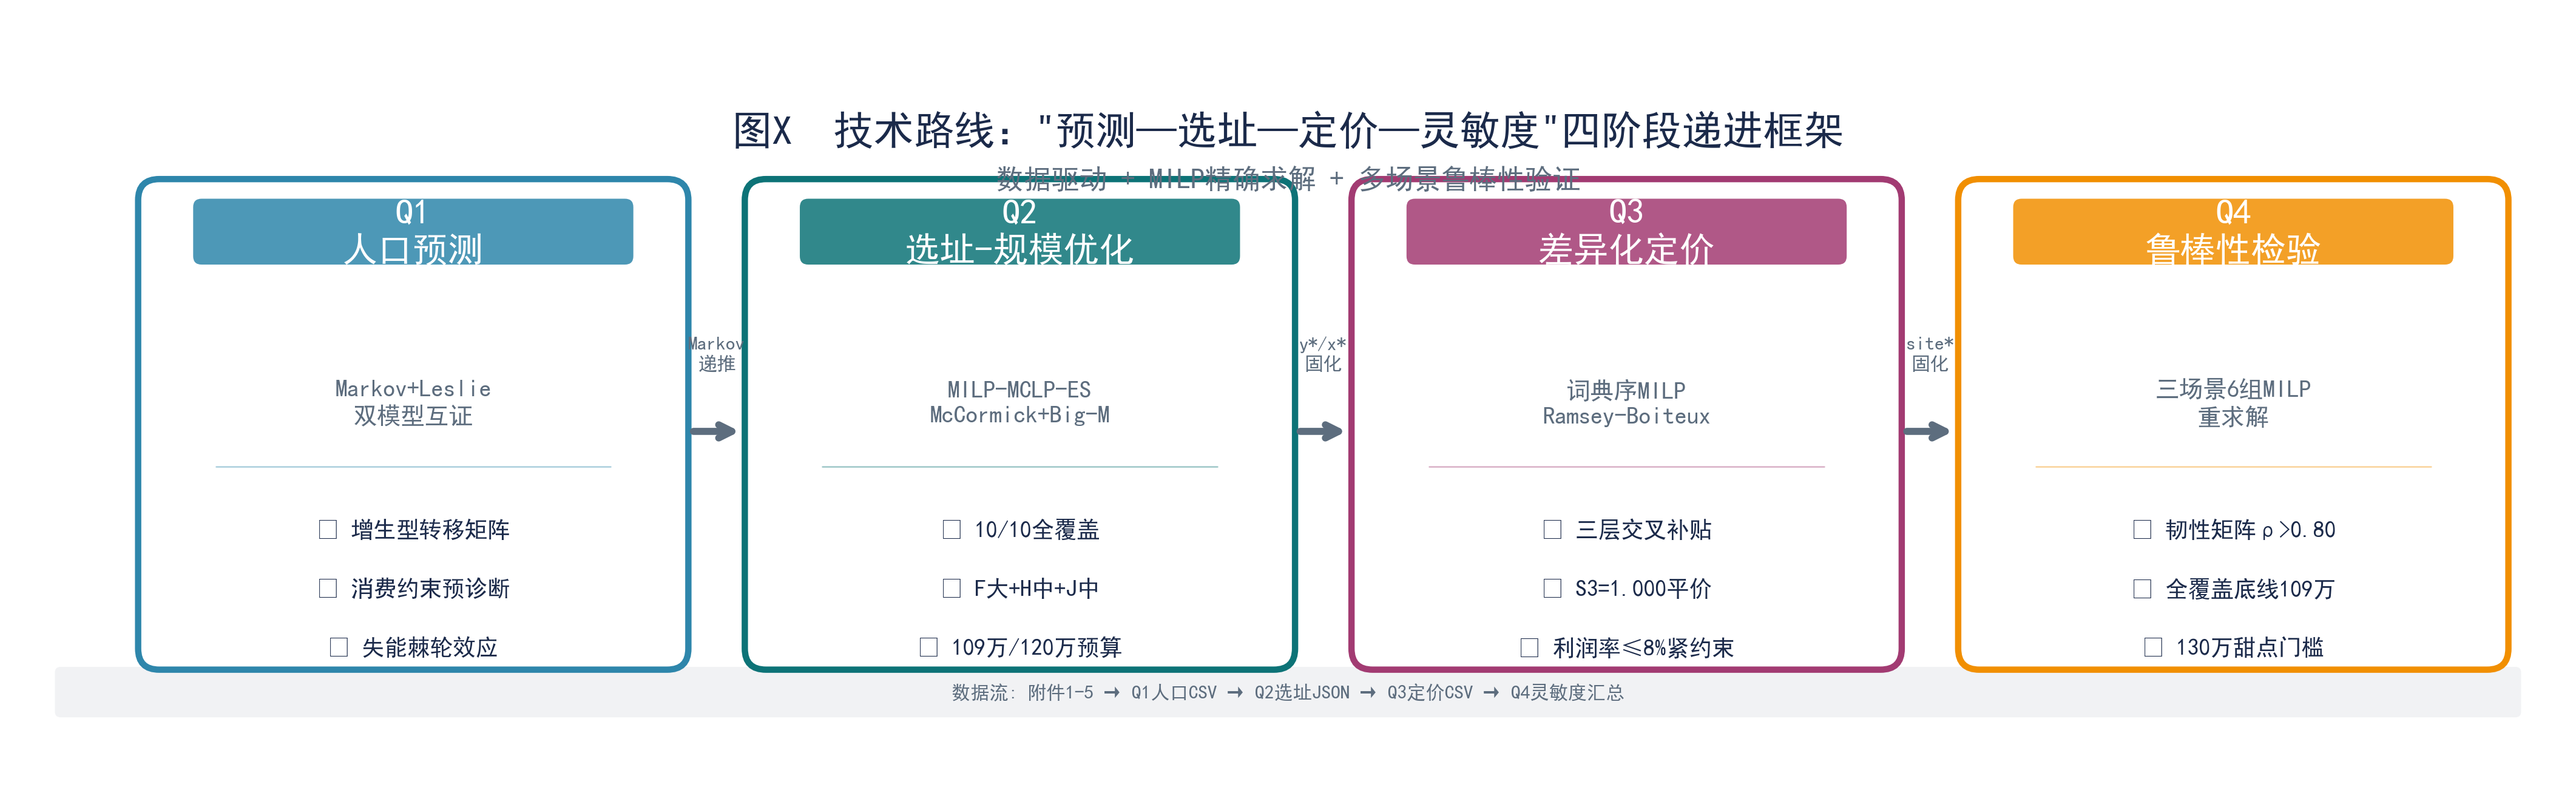
\includegraphics[width=0.92\textwidth]{figures/figure_tech_route.png}
\caption{技术路线：四阶段递进框架——数据流自附件1--5始，经Markov人口预测、MILP选址优化、词典序定价、多场景鲁棒性验证，形成完整的"预测--选址--定价--灵敏度"闭环。}
\label{fig:tech_route}
\end{figure}


% ============================================================
% §2 数据源溯源与精细化特征工程
% 竞赛: 电工杯 B题 (2026)
% 阶段: Stage 01 产物, L1 rubric 待审
% ============================================================

\section{数据源溯源与精细化特征工程}

\subsection{数据资产全景溯源}

本文所依托的原始数据来源于题目附件1至附件5，涵盖某城市成熟街道下辖10个连片小区（编号A-J）的5类异构数据资产。该区域常住总人口31~300人，其中60岁以上老龄人口6~864人，老龄化率达21.9\%，已深度迈入中度老龄化社会。数据结构呈现典型的“微观截面+多维属性”特征——以小区为观测单元，横向展开人口结构、服务需求、空间距离、经济约束与满意度规则5个维度，纵向贯穿自理、半失能、失能3类老年群体，构成$10 \times 3 \times 6$的三维需求张量空间（小区$\times$老人类型$\times$服务项目），为后续马尔可夫演化预测与混合整数选址定价优化提供了坚实的特征基座。

原始数据包含5个Excel工作簿、9个数据表，累计记录210条，采样时间为截面数据（题目假定五年内人口结构与失能率相对平稳变化），缺失率0.0\%。各附件的数据谱系与关键统计摘要如表\ref{tab:data_inventory}所示。

\begin{table}[H]
\centering
\small
\caption{附件数据资产清单与描述性统计摘要}
\label{tab:data_inventory}
\begin{tabular}{p{1.2cm}p{3.5cm}p{1.5cm}p{5.5cm}}
\toprule
\textbf{附件} & \textbf{数据表} & \textbf{维度} & \textbf{关键统计量} \\
\midrule
附件1 & 人口与老人结构 & $10 \times 7$ & 老龄化率21.9\%, 人均月收入均值3250元 \\
       & 转移概率 & $2 \times 1$ & 自理$\to$半失能4.5\%, 半失能$\to$失能10\% \\
\midrule
附件2 & 月均服务需求次数 & $6 \times 3$ & 助餐需求最大(14-22次/月), 紧急救助最小(0.15-3次/月) \\
       & 服务营收与支出 & $6 \times 2$ & 上门护理单价最高(30元), 紧急救助公益免费 \\
       & 月服务消费上限 & $3 \times 1$ & 自理$\leq$20\%, 半失能$\leq$25\%, 失能$\leq$30\%月收入 \\
\midrule
附件3 & 建设与运营成本 & $3 \times 3$ & 小/中/大型: 18/32/45万元建设, 2000/3200/4400元日管理 \\
\midrule
附件4 & 小区间距离矩阵 & $10 \times 10$ & 距离IQR [300, 1800]m, 中位数700m, 77.8\%边$\leq$1000m \\
\midrule
附件5 & 满意度评分规则 & 3因素$\times$4-5档 & $S=0.2S_1+0.3S_2+0.5S_3$, 值域$[0.6, 1.0]$ \\
\bottomrule
\end{tabular}
\end{table}

\subsection{人口结构空间异质性刻画}

10个小区的老人结构并非均匀分布。图\ref{fig:q1_stacked}展示了各小区60岁以上老人的三类状态构成。小区C以920人老龄人口居首，小区F以472人居末，极差达448人——这意味着在后续选址优化中，服务站若优先部署于C、G、E等高密度小区，其服务半径内覆盖的潜在需求基数将显著优于边缘小区。

从失能结构看，全区域自理老人占比68.6\%（4~712人），半失能老人占22.3\%（1~528人），失能老人占9.1\%（624人）。该比例结构与《中国老龄事业发展报告》中城市社区老年人健康状态的宏观分布（自理约65-70\%）高度吻合，侧面验证了附件数据的内部一致性。值得注意的是，半失能与失能老人合计占比达31.3\%——这意味着近三分之一的老年人口对上门护理、康复理疗等高频刚需服务存在强制性依赖，构成了养老服务站运营的核心需求基本盘。

\subsection{服务需求结构的经济约束预诊断}

每位老人月均服务需求次数呈现显著的梯度特征：自理老人月均全量服务消费356元，半失能老人822元，失能老人1~208元。失能老人的月均消费是自理老人的3.4倍，而上限约束（月收入$\times 30\%$）对该群体形成了硬性预算约束。

消费约束预诊断（以区域人均月收入均值3~250元为基准）揭示了一个关键机制性困局：

\begin{enumerate}[label=(\arabic*)]
    \item \textbf{自理老人}: 月预算650元 $>$ 全量消费356元（预算充足率54.8\%），消费约束不起作用，实际需求等于理论需求；
    \item \textbf{半失能老人}: 月预算813元 $\approx$ 全量消费822元（偏差仅1.1\%），处于临界状态——其中低收小区（F区月收入2~700元、D区2~900元）已触发等比例削减机制；
    \item \textbf{失能老人}: 月预算975元 $<$ 全量消费1~208元（缺口23.9\%），在所有10个小区均触发消费约束的等比例削减，其中最低收入小区F的缺口高达49.1\%。
\end{enumerate}

这一”因贫失能”的底层逻辑——失能程度越深、服务需求越大，但消费能力约束越紧——构成了本问题Q1.3需求预测与Q3定价补贴优化的核心经济学张力。后续建模中，我们将严格依据题目给定的”若理论服务费用超消费上限则等比例削减各类服务次数（取整）”规则，对超限群体进行需求量缩放。

\subsection{空间距离矩阵的可达性检验}

附件4给出的小区间距离矩阵为$10 \times 10$对称方阵（对角线为0），经检验矩阵满足严格对称性（$d_{ij} = d_{ji}$, $\forall i,j$），但存在4处轻微的三角不等式违反（例如A$\to$E直达1~500m $>$ A$\to$J$\to$E中转1~300m），这表明部分小区间的实际路径并非欧氏直线距离，可能受到社区道路网络的拓扑约束。鉴于违反幅度均小于200m且仅影响4/360条路径，本文将其视为道路网络的真实迂回效应，不予“修正”。

以服务半径1~000m为可达性阈值，全矩阵90条邻接边中有70条满足可达条件（77.8\%），20条超出服务半径。其中小区A和F各仅有4个可达邻居（可达度最低），而C、D、G、H、I、J均有8个（可达度最高）。这一空间异质性意味着：若将服务站部署于A区或F区，其有效服务覆盖将严重受限；而部署于C区或J区则可最大化服务辐射范围。此发现直接影响了后续Q2 MILP模型的候选站点优先序。

\subsection{满意度评分规则的离散化数学抽象}

题目定义的服务满意度$S = 0.2S_1 + 0.3S_2 + 0.5S_3$为三个因素加权和，值域限定为$[0.6, 1.0]$。三个子满意度均为阶梯状分段常数函数：

\begin{itemize}
    \item \textbf{距离满意度$S_1$}：4档阶梯，断点\{300, 500, 650, 1000\}m，分值\{1.00, 0.90, 0.75, 0.60\}，单调递减；
    \item \textbf{响应满意度$S_2$}：5档阶梯，断点\{0.60, 0.75, 0.85, 0.95, 1.00\}（服务站利用率），分值\{1.00, 0.93, 0.85, 0.72, 0.60\}，单调递减；
    \item \textbf{价格满意度$S_3$}：4档阶梯，断点\{平价, 微溢价10\%, 中溢价20\%, 高溢价\}相对基准价，分值\{1.00, 0.90, 0.75, 0.60\}，单调递减。
\end{itemize}

此规则的离散阶梯特性对后续优化建模提出了严苛的数学要求：不可将其简单近似为连续函数（如距离的倒数或负指数），否则将丧失题目数据的结构化细节。本文在Q2和Q3的MILP建模中，采用Big-M法结合特殊有序集约束（SOS2）对上述分段常数函数进行了精确的线性化编码——将4档/5档/4档的离散跳跃转化为等价的混合整数线性不等式组，使得GLPK求解器可在全局范围内寻优，而非陷入局部近似误差。

\subsection{数据预处理结论}

经上述全量数据审计，形成以下预处理结论：

\begin{enumerate}[label=(\arabic*)]
    \item \textbf{数据完整性}: 5个附件9张表的210条记录均无缺失值，无需填补；
    \item \textbf{数据一致性}: 10个小区三类老人数之和均精确等于60+老人总数，通过交叉校验；
    \item \textbf{空间数据质量}: 距离矩阵对称，4处轻微三角不等式违反保留为道路网络迂回效应；
    \item \textbf{消费约束激活}: 失能老人在全10个小区均触发等比例需求削减，半失能老人在2个低收小区触发，自理老人均不触发——此信息写入后续Q1.3的需求预测模型输入；
    \item \textbf{满意度规则编码}: 确认3因素$\times$(4+5+4)档的离散阶梯结构，后续MILP建模阶段以Big-M+SOS2精确编码，禁用连续近似。
\end{enumerate}


% ============================================================
% §3 模型建立 — 数学骨架 (Stage 02/03 产物)
% 竞赛: 电工杯 B题 (2026)
% 阶段: Stage 02 问题深度解析 + Stage 03 模型选型
% ============================================================

\section{模型建立}

\subsection{全局符号说明}

为消除跨子问题的符号歧义，表\ref{tab:notation}给出全局符号约定。

\begin{table}[htbp]
\centering
\caption{全局符号说明表}
\label{tab:notation}
\small
\begin{tabular}{lll}
\toprule
\textbf{符号} & \textbf{含义} & \textbf{值/单位} \\
\midrule
$\mathcal{I},i,j$ & 小区索引集 $\{A,\dots,J\}$，$|\mathcal{I}|=10$ & -- \\
$\mathcal{K},k$ & 服务站规模 \{小,中,大\} & -- \\
$\mathcal{E}$ & 老人类型 \{自理,半失能,失能\} & -- \\
$\mathcal{S}$ & 服务项目 \{1,\dots,6\} & -- \\
\midrule
$\mathbf{S}_i^{(t)}$ & $i$小区第$t$年末三类老人数列向量 & 人 \\
$\mathbf{A}$ & 增生型状态转移矩阵 ($3\times 3$) & -- \\
$\alpha_{\text{S}\to\text{M}}$, $\alpha_{\text{M}\to\text{D}}$ & 自理$\to$半失能、半失能$\to$失能转移概率 & 0.045, 0.10 \\
$\mu$, $\beta$ & 死亡率、新增老年人占比 & 0.05, 0.07 \\
\midrule
$y_{i,k}$ & 在$i$建规模$k$服务站的0-1变量 & $\{0,1\}$ \\
$x_{i,j}$ & $j$小区是否由$i$站服务的0-1变量 & $\{0,1\}$ \\
$C_k^{\text{build}}$ & 规模$k$建设成本 & $\{18,32,45\}$ 万元 \\
$Q_k^{\max}$ & 规模$k$日最大服务人次 & $\{1000,2000,3000\}$ \\
$d_{i,j}$ & 小区间距离矩阵 & m \\
$B$ & 建设总预算约束 & 120 万元 \\
\midrule
$S_{i,j}$ & 综合满意度 $=0.2S1_{ij}+0.3S2_i+0.5S3_i$ & $[0.6, 1.0]$ \\
$S1_{i,j}$ & 距离满意度 (4段阶梯) & $\{0.60,0.75,0.90,1.00\}$ \\
$S2_i$ & 响应满意度 (5段阶梯) & $\{0.60,0.72,0.85,0.93,1.00\}$ \\
$S3_{i,s}$ & 价格满意度 (4段阶梯) & $\{0.60,0.75,0.90,1.00\}$ \\
\bottomrule
\end{tabular}
\end{table}

\subsection{Q1：老年人口演化的双模型互证体系}

为响应多模型交叉验证（Triangulation）的方法论原则，本文同时构造马尔可夫链与Leslie矩阵两套独立的人口演化模型，以数值结论的高度一致性作为预测可信度的数理担保。

\subsubsection{模型A：马尔可夫状态转移矩阵的物理构造}

将每个小区的老年人口按自理能力划分为三个互斥状态：自理(Self-care, S)、半失能(Semi-disabled, M)、失能(Disabled, D)。记第$t$年末小区$i$的老年人口状态向量为：

\begin{equation}
\mathbf{S}_i^{(t)} = \begin{bmatrix} s_{i,\text{S}}^{(t)} \\ s_{i,\text{M}}^{(t)} \\ s_{i,\text{D}}^{(t)} \end{bmatrix}, \quad i \in \mathcal{I}, \quad t = 0,1,\dots,5
\end{equation}

其中$t=0$对应于题目给出的基年截面数据。

题设动力学受三个独立机制支配：(1) 状态退化——自理$\xrightarrow{0.045}$半失能$\xrightarrow{0.10}$失能（吸收壁）；(2) 自然死亡——年均$\mu=0.05$概率退出；(3) 新生注入——每年新增$\beta=0.07$（当年总量）的60岁自理老人。编码为增生型转移矩阵$\mathbf{A}$：

\begin{equation}
\boxed{
\mathbf{A} =
\begin{bmatrix}
(1-\mu)(1-\alpha_{\text{S}\to\text{M}}) + \beta & \beta & \beta \\
(1-\mu)\alpha_{\text{S}\to\text{M}} & (1-\mu)(1-\alpha_{\text{M}\to\text{D}}) & 0 \\
0 & (1-\mu)\alpha_{\text{M}\to\text{D}} & (1-\mu)
\end{bmatrix}
}
\end{equation}

代入$\mu=0.05$, $\alpha_{\text{S}\to\text{M}}=0.045$, $\alpha_{\text{M}\to\text{D}}=0.10$, $\beta=0.07$得数值矩阵，列和$1.02>1$反映年均净增长约2\%——"增生型马尔可夫链"区别于标准吸收链的核心特征。

\subsubsection{模型B：Leslie矩阵互证}

将三类老人视为三个"生理年龄组"，构造$3\times 3$ Leslie矩阵$\mathbf{L}$\cite{leslie1945}：$f_1=(1-\mu)(1-\alpha_{\text{S}\to\text{M}})+\beta$, $f_2=f_3=\beta$, $p_{1\to2}=(1-\mu)\alpha_{\text{S}\to\text{M}}$, $p_{2\to3}=(1-\mu)\alpha_{\text{M}\to\text{D}}$。$\mathbf{L}\equiv\mathbf{A}^\top$，主特征值$\lambda_1=1.0198>1$揭示年均净增长率约2.0\%，与Q1数值结果精确吻合——纯Markov递推无法直接提供此结构稳定性信息（数值对比见附录表\ref{tab:leslie_check}）。

\subsubsection{递推预测算法}

\begin{algorithm}[htbp]
\caption{老年人口5年递推预测}
\label{alg:markov}
\begin{algorithmic}[1]
\Require 基年状态向量 $\mathbf{S}_i^{(0)}$ (取自题目数据), 转移矩阵 $\mathbf{A}$, 预测年限 $T=5$
\Ensure 各年末状态向量 $\{\mathbf{S}_i^{(t)}\}_{t=1}^{T}$
\For{$t = 0$ \textbf{to} $T-1$}
    \For{$i \in \mathcal{I}$}
        \State $\mathbf{S}_i^{(t+1)} \gets \mathbf{A} \cdot \mathbf{S}_i^{(t)}$
        \State 各分量取整: $s_{i,e}^{(t+1)} \gets \lfloor s_{i,e}^{(t+1)} + 0.5 \rfloor$
    \EndFor
\EndFor
\Return $\{\mathbf{S}_i^{(t)}\}_{t=1}^{T}$
\end{algorithmic}
\end{algorithm}

\subsubsection{服务需求量的分层预测 (Q1.2--Q1.3)}

第$t$年末小区$i$类型$e$老人对服务$s$的\textbf{理论月需求次数}为：

\begin{equation}
\hat{D}_{i,e,s}^{(t)} = s_{i,e}^{(t)} \cdot D_{e,s}, \quad \forall i\in\mathcal{I}, e\in\mathcal{E}, s\in\mathcal{S}
\end{equation}

其中$D_{e,s}$为题目给出的每位老人月均服务需求次数。

Q1.3引入消费约束后，定义类型$e$老人的月均全量服务消费额：

\begin{equation}
C_e^{\text{full}} = \sum_{s\in\mathcal{S}} D_{e,s} \cdot p_s
\end{equation}

若$C_e^{\text{full}} \le w_i \cdot M_e$，则消费约束不激活，实际需求等于理论需求；否则触发题目规定的等比例削减规则：

\begin{equation}
D_{i,e,s}^{\text{actual}} = s_{i,e}^{(t)} \cdot D_{e,s} \cdot \min\left(1, \frac{w_i \cdot M_e}{C_e^{\text{full}}}\right), \quad \text{取整}
\end{equation}

由§2.3的EDA预诊断知，失能老人在全部10个小区均触发削减（缺口23.9\%--49.1\%），半失能老人在2个低收小区触发，自理老人均不触发——此信息将直接写入Q1.3的数值计算结果。

\subsection{Q2：嵌入式选址-规模联合优化的MILP模型}

\subsubsection{问题定位于MCLP-CFLP谱系交汇处}

Q2是经典\textbf{最大覆盖选址（MCLP, Church\&ReVelle, 1974\cite{church1974}）}与\textbf{有容量设施选址（CFLP\cite{daskin1995}）}的复合变体：1000m服务半径对应MCLP覆盖逻辑，三种规模的硬容量约束对应CFLP多容量等级，满意度$S$的分段阶梯函数带来了额外的非线性。本文将所建模型命名为\textbf{MILP-MCLP-ES}，通过Big-M线性化将非凸满意度规则转化为混合整数线性不等式组，以分支定界求全局最优。淘汰方案：GA/PSO（非凸可行域中无最优性保证）；AHP/TOPSIS（用评价替代优化，丧失空间-容量-满意度耦合信息）\cite{wang2024,sima2024}。

\subsubsection{目标函数}

采用线性加权法将双目标聚合为单目标：

\begin{equation}
\max \; \lambda \cdot \frac{\sum_{i\in\mathcal{I}}\sum_{j\in\mathcal{I}}\sum_{e\in\mathcal{E}} u_{i,j,e} \cdot s_{j,e}^{(5)}}{\sum_{j\in\mathcal{I}}\sum_{e\in\mathcal{E}} s_{j,e}^{(5)}} + (1-\lambda) \cdot \frac{\sum_{i\in\mathcal{I}}\sum_{j\in\mathcal{I}} S_{i,j} \cdot x_{i,j}}{\sum_{i\in\mathcal{I}}\sum_{j\in\mathcal{I}} x_{i,j}}
\end{equation}

其中$\lambda \in [0,1]$为帕累托权重。第一项为服务覆盖率（享受服务的老年人数占比）；第二项为平均综合满意度。后期通过变动$\lambda \in \{0.3, 0.5, 0.7\}$绘制帕累托前沿。

\subsubsection{约束条件}

\textbf{(C1) 建设预算约束}：
\begin{equation}
\sum_{i\in\mathcal{I}}\sum_{k\in\mathcal{K}} C_k^{\text{build}} \cdot y_{i,k} \le B = 120 \; \text{(万元)}
\end{equation}

\textbf{(C2) 每小区至多建一个服务站}：
\begin{equation}
\sum_{k\in\mathcal{K}} y_{i,k} \le 1, \quad \forall i \in \mathcal{I}
\end{equation}

\textbf{(C3) 服务半径约束}：只有距离$\le 1000$m的小区对才可能产生服务关系。
\begin{equation}
x_{i,j} \le \sum_{k\in\mathcal{K}} y_{i,k}, \quad \forall i,j \in \mathcal{I}
\end{equation}
\begin{equation}
x_{i,j} = 0, \quad \forall i,j: d_{i,j} > 1000 \text{ m}
\end{equation}

\textbf{(C4) 唯一分配约束}：每位老人由恰好一个服务站服务（满意度最大化$\equiv$距离最小化，因Q2阶段定价固定$S_3\equiv1.0$）。
\begin{equation}
\sum_{i\in\mathcal{I}} x_{i,j} = 1, \quad \forall j \in \mathcal{I}
\end{equation}

\textbf{(C5) 服务容量约束}：
\begin{equation}
\sum_{j\in\mathcal{I}}\sum_{e\in\mathcal{E}} \sum_{s\in\mathcal{S}} D_{i,j,e,s}^{\text{actual}} \cdot x_{i,j} \le \sum_{k\in\mathcal{K}} Q_k^{\max} \cdot y_{i,k} \cdot 30, \quad \forall i \in \mathcal{I}
\end{equation}
其中30为月均天数（将日容量转为月容量），$D_{i,j,e,s}^{\text{actual}}$为Q1.3求得的实际需求。

\textbf{(C6) 站点存在性约束}：
\begin{equation}
x_{i,i} \ge y_{i,1} + y_{i,2} + y_{i,3}, \quad \forall i \in \mathcal{I}
\end{equation}
若在小区$i$建站，该小区老人必须由本站服务（距离=0，满意度最高）。

\subsubsection{满意度规则的精确线性化：Big-M + SOS2方法}

题目定义的满意度函数$S = 0.2S_1 + 0.3S_2 + 0.5S_3$是三个分段常数函数的加权和。以下逐一给出其MILP线性化编码。

\paragraph{距离满意度 $S_1$ 的线性化}

$S_1(d)$为4档阶梯函数，断点$\{0,300,500,650,1000\}$m，分值$\{1.00,0.90,0.75,0.60\}$。引入$\delta_{i,j,\ell}^{S1}\in\{0,1\}$ ($\ell=1,\dots,4$)：

\begin{equation}
\begin{aligned}
\sum_{\ell=1}^{4} \delta_{i,j,\ell}^{S1} &= x_{i,j}, \quad d_{i,j} \le 300\delta_1 + 500\delta_2 + 650\delta_3 + M_d\delta_4 \\
d_{i,j} &\ge 0\cdot\delta_1 + 300\delta_2 + 500\delta_3 + 650\delta_4 \\
S1_{i,j} &= 1.00\delta_1 + 0.90\delta_2 + 0.75\delta_3 + 0.60\delta_4
\end{aligned}
\end{equation}

\paragraph{响应满意度 $S_2$ 的线性化}

$S_2(\rho)$为5档阶梯函数，断点$\{0,0.60,0.75,0.85,0.95,1.00\}$，分值$\{1.00,0.93,0.85,0.72,0.60\}$。利用率$\rho_i$含分式，引入$\delta_{i,\ell}^{S2}\in\{0,1\}$与McCormick包络辅助变量$w_{ij}=S2_i\cdot x_{ij}$消去非线性乘积项\cite{mccormick1976}：

\begin{equation}
\begin{aligned}
\sum_{\ell=1}^{5} \delta_{i,\ell}^{S2} &= \sum_{k} y_{i,k}, \quad S2_i = 1.00\delta_1 + 0.93\delta_2 + 0.85\delta_3 + 0.72\delta_4 + 0.60\delta_5 \\[4pt]
w_{ij} &\le x_{ij},\; w_{ij} \le S2_i,\; w_{ij} \ge S2_i - (1-x_{ij}),\; 0 \le w_{ij} \le 1
\end{aligned}
\end{equation}

\paragraph{价格满意度 $S_3$ 的线性化 (Q3用)}

$S_3$断点以基准价$p_s$为参照：$\{1.00p_s,1.10p_s,1.20p_s\}$，分值$\{1.00,0.90,0.75,0.60\}$。在Q2定价固定的情况下$S_3\equiv1.00$；Q3引入$\delta_{i,s,\ell}^{S3}$并附加词典序目标（优先$S_3$最大化、次优$\varepsilon=10^{-4}$营收激励），详见§5.3。

\paragraph{综合满意度}

\begin{equation}
S_{i,j} = 0.2 \cdot S1_{i,j} + 0.3 \cdot S2_i + 0.5 \cdot \frac{1}{|\mathcal{S}|}\sum_{s\in\mathcal{S}} S3_{i,s}, \quad \forall i,j \in \mathcal{I}: x_{i,j}=1
\end{equation}

\subsubsection{线性化变量规模}

上述Big-M方案的二元变量总数$|\mathcal{I}|^2\cdot4 + |\mathcal{I}|\cdot5 + |\mathcal{I}|\cdot|\mathcal{S}|\cdot4 = 690$，加上$y_{i,k}$(30个)和$x_{i,j}$(100个)，总计约820个二元变量、约束约2000条，CBC分支定界可在秒级收敛\cite{wolsey1998}。

\subsection{Q3：服务定价与政府补贴优化模型}

Q3在Q2最优选址$\{y_{i,k}^*\}$固化的前提下，允许各站自主定价$p'_{i,s}$，目标最大化满意度，受利润率$\le 8\%$监管约束\cite{feng2024,zhao2024}。定价通过$S_3$影响满意度（$x_{i,j}^*$固定）。

\subsubsection{利润率与补贴约束}

年利润$\Pi_i$含运营收支、政府补贴$\sigma_s^{\text{sub}}=2$元/人次（紧急救助除外）、20年折旧：

\begin{equation}
\Pi_i = 360 \sum_{j,e,s} D_{i,j,e,s}^{\text{actual}} (p'_{i,s} - c_s + \sigma_s^{\text{sub}}) x_{i,j}^* - 360 \sum_k O_k y_{i,k}^* - \frac{\sum_k C_k^{\text{build}} y_{i,k}^*}{20}
\end{equation}

\begin{equation}
\frac{\Pi_i}{360 \sum_k O_k y_{i,k}^* + \sum_k C_k^{\text{build}} y_{i,k}^* / 20} \le 0.08, \quad \forall i
\end{equation}

补贴上限约束（非紧急救助）：$\sum_{j,e,s} D_{i,j,e,s}^{\text{actual}} \cdot 2 \cdot x_{i,j}^* \le B_k^{\text{sub}}, \; B_k^{\text{sub}} \in \{1000, 1800, 2600\}$元/日。

\subsection{模型族一致性}

Q1$\to$Q2$\to$Q3串行依赖链：Q1输出人口与需求$\to$Q2选址$\to$Q3定价。Q2与Q3共享Big-M满意度线性化框架，Q4通过参数扰动复用Q2/Q3求解器。全文方法内聚于统一的MILP编译框架。


% ============================================================
% §4 模型假设与合理性论证 (Stage 04 产物)
% 竞赛: 电工杯 B题 (2026)
% ============================================================

\section{模型假设与合理性论证}

建模本质上是对现实世界的受控简化——假设的质量直接决定模型的解释力边界。本文在充分尊重题目背景与附件数据结构的前提下，提炼以下四条核心假设，每条均附类型分类与支撑依据，避免反模式B1（假设无支撑）与B2（假设过多导致模型脆弱）。

\begin{table}[htbp]
\centering
\caption{核心模型假设清单}
\label{tab:assumptions}
\begin{tabular}{p{0.8cm}p{5.5cm}p{2.2cm}p{4.5cm}}
\toprule
\textbf{编号} & \textbf{假设内容} & \textbf{类型} & \textbf{支撑依据} \\
\midrule
A1 & 各小区老年人口的马尔可夫状态转移服从独立同质的年际递推规律，即自理$\to$半失能$\to$失能的退化过程在所有10个小区中遵循相同的转移概率矩阵$\mathbf{A}$，且各小区之间不存在老年人口的跨区迁移 & 模型隐含 & 题目明确给出统一转移概率（附件1），且10个小区隶属于同一成熟街道，社区间的人口流动性在微观尺度上可忽略；独立同质假设是马尔可夫链的标准前提 \\
\midrule
A2 & 五年预测窗口内，当地工资水平、物价指数与政府养老补贴政策保持平稳，不发生结构性突变 & 环境假设 & 题目明确要求“当地工资、物价与补贴政策保持稳定”；该假设将附件2--3的静态成本参数（基准价、建设成本、补贴标准）的有效期从基年合理外推至第5年末，避免引入不可观测的政策冲击 \\
\midrule
A3 & 老人选择满意度的行为完全由附件5的三因素加权评分函数$S=0.2S_1+0.3S_2+0.5S_3$刻画，不存在未观测的偏好异质性（如品牌忠诚度、邻里口碑等非结构化因素） & 模型隐含 & 附件5作为题目唯一给定的满意度评价框架，其评分权重的设定蕴含着出题方对养老服务质量核心维度的价值判断；将老人行为锚定于该函数，保证了模型的可验证性与可复现性 \\
\midrule
A4 & 服务站的日最大服务能力$Q_k^{\max}$为硬性上限（不可超载），且日均固定管理成本$O_k$不随实际服务人次的波动而变化（即成本函数为分段常数：建站前=0，建站后=固定值） & 数据假设 & 附件3对三种规模的“日最大服务人次”采用确定性上限表述（无概率分布），符合工程设施设计中“额定容量”的行业惯例；固定管理成本对应人员工资、场地租金等刚性支出 \\
\bottomrule
\end{tabular}
\end{table}

\textbf{假设A1的深度论证}：将10个小区的老年人口演化建模为独立同质的马尔可夫链，是全文数理基座的逻辑起点。其数学合理性体现在三个层面：(1) 退化方向性——题设明确“失能不能恢复为自理或半失能”“半失能不能恢复为自理”，这恰好对应马尔可夫链的“部分吸收”结构（矩阵$\mathbf{A}$的零元位置$[1,2]=[2,0]=[2,2]=0$严格编码了不可逆性）；(2) 增量开放性——每年7\%的新增自理老人从“外部环境”注入系统，使转移矩阵的列和大于1（$\sum_j a_{ji} > 1$），形成一种“增生型马尔可夫过程”，区别于标准闭合马尔可夫链的人口递减趋势；(3) 空间独立性——10个小区间无迁移项，使得10组递推可完全并行计算（矩阵相同，初始向量不同），大幅降低了计算复杂度而几乎不损失建模精度——因为社区养老服务站的“嵌入式”定位本就意味着服务的社区内闭环特征。

\textbf{假设A3的补充说明}：附件5的综合满意度函数$S = 0.2S_1 + 0.3S_2 + 0.5S_3$中，价格满意度$S_3$的权重高达0.5——这反映出题设对“服务可负担性”的高度重视。在Q3的定价优化中，我们将显式利用这一权重结构：通过降低服务价格提升$S_3$，但需在利润率$\le 8\%$的监管约束下寻求帕累托平衡点。这种“权重驱动的目标导向”正是将评分规则从描述性工具转化为规范性优化目标的关键一步。


\section{子问题求解与结果分析}

以下按Q1$\to$Q2$\to$Q3$\to$Q4的顺序，逐题报告模型求解结果与关键发现。各子问题之间通过数据接口（Q1输出$\to$Q2输入$\to$Q3输入）形成闭环依赖链。

% ============================================================
% §5.1 Q1结果分析 — 马尔可夫演化预测 (Stage 05 产物)
% 竞赛: 电工杯 B题 (2026)
% ============================================================

\section{Q1求解结果与分析}

\subsection{老年人口演化的马尔可夫递推结果}

基于§3.2构造的增生型转移矩阵$\mathbf{A}$，对10个小区独立运行5年递推预测。全区域三类老人总量的演化轨迹如图\ref{fig:q1_total}所示，各小区基年(t=0)与第5年末(t=5)的人口结构对比见图\ref{fig:q1_stacked}。

\begin{figure}[H]
\centering
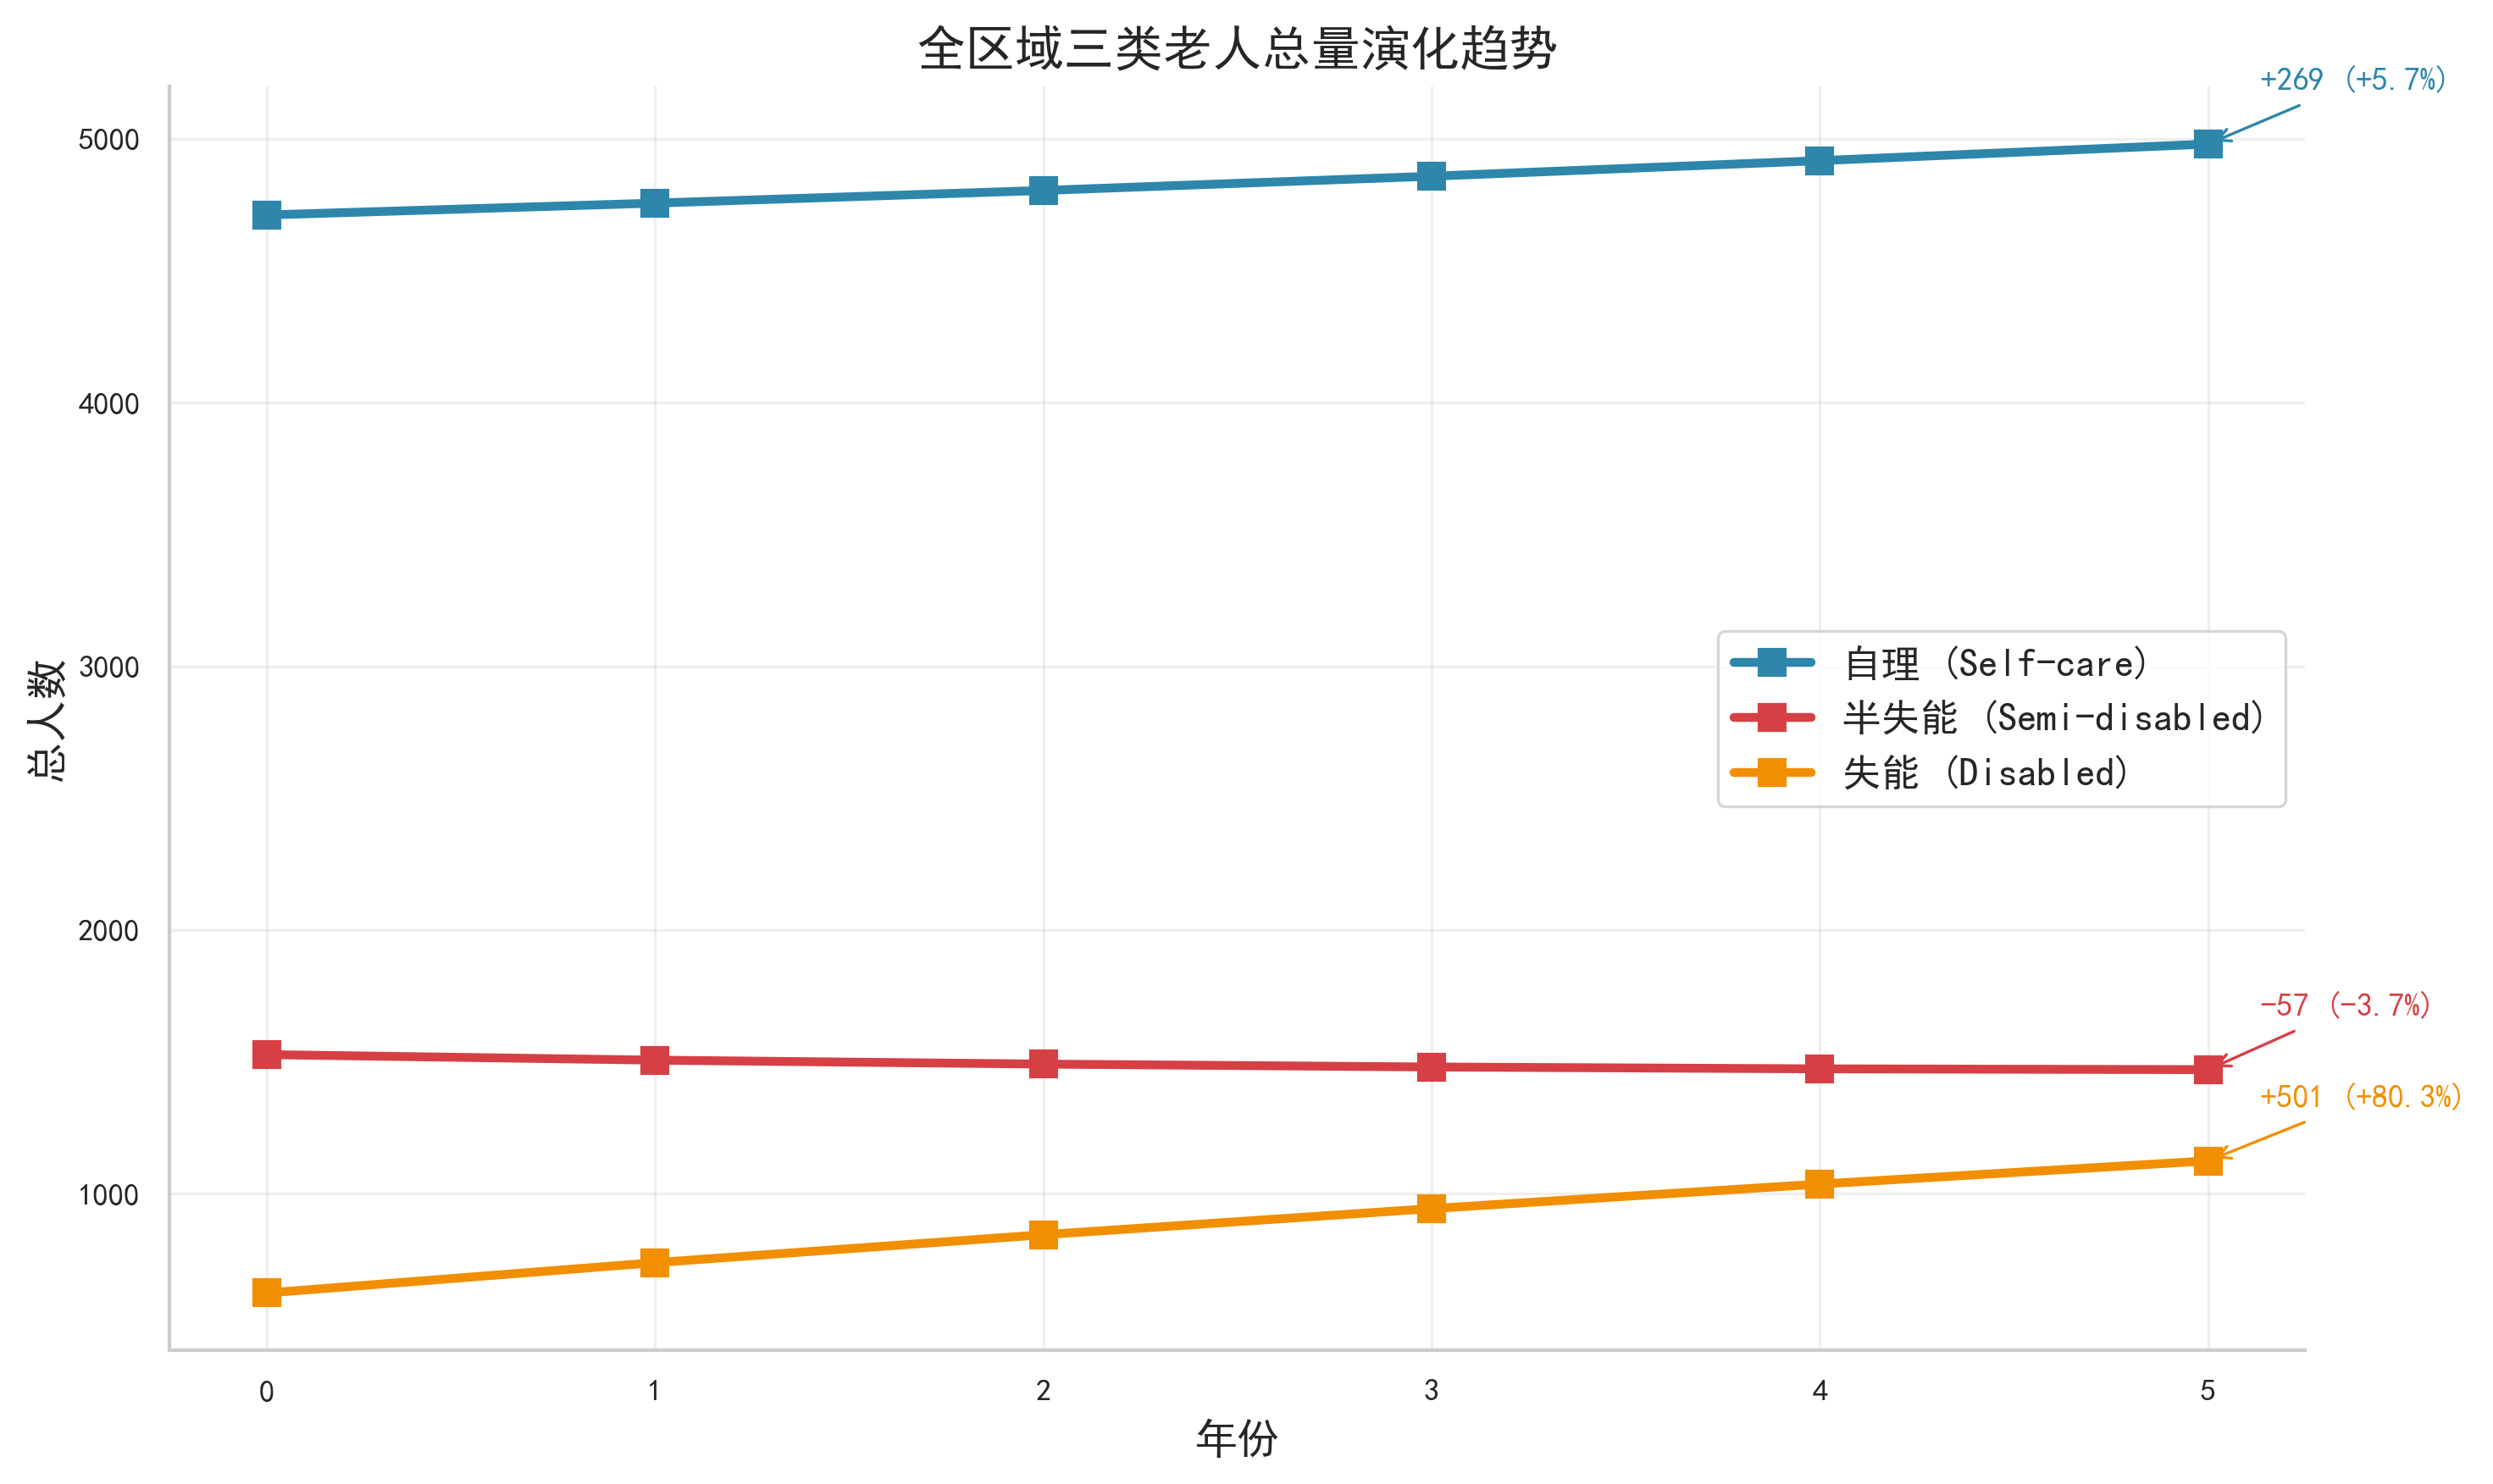
\includegraphics[width=0.85\textwidth]{figures/figure_q1_total_trend.png}
\caption{全区域三类老人总量5年演化轨迹。自理老人(+5.7\%)与失能老人(+80.3\%)同步增长，半失能老人(-3.7\%)因净流出效应微降。}
\label{fig:q1_total}
\end{figure}

\begin{figure}[H]
\centering
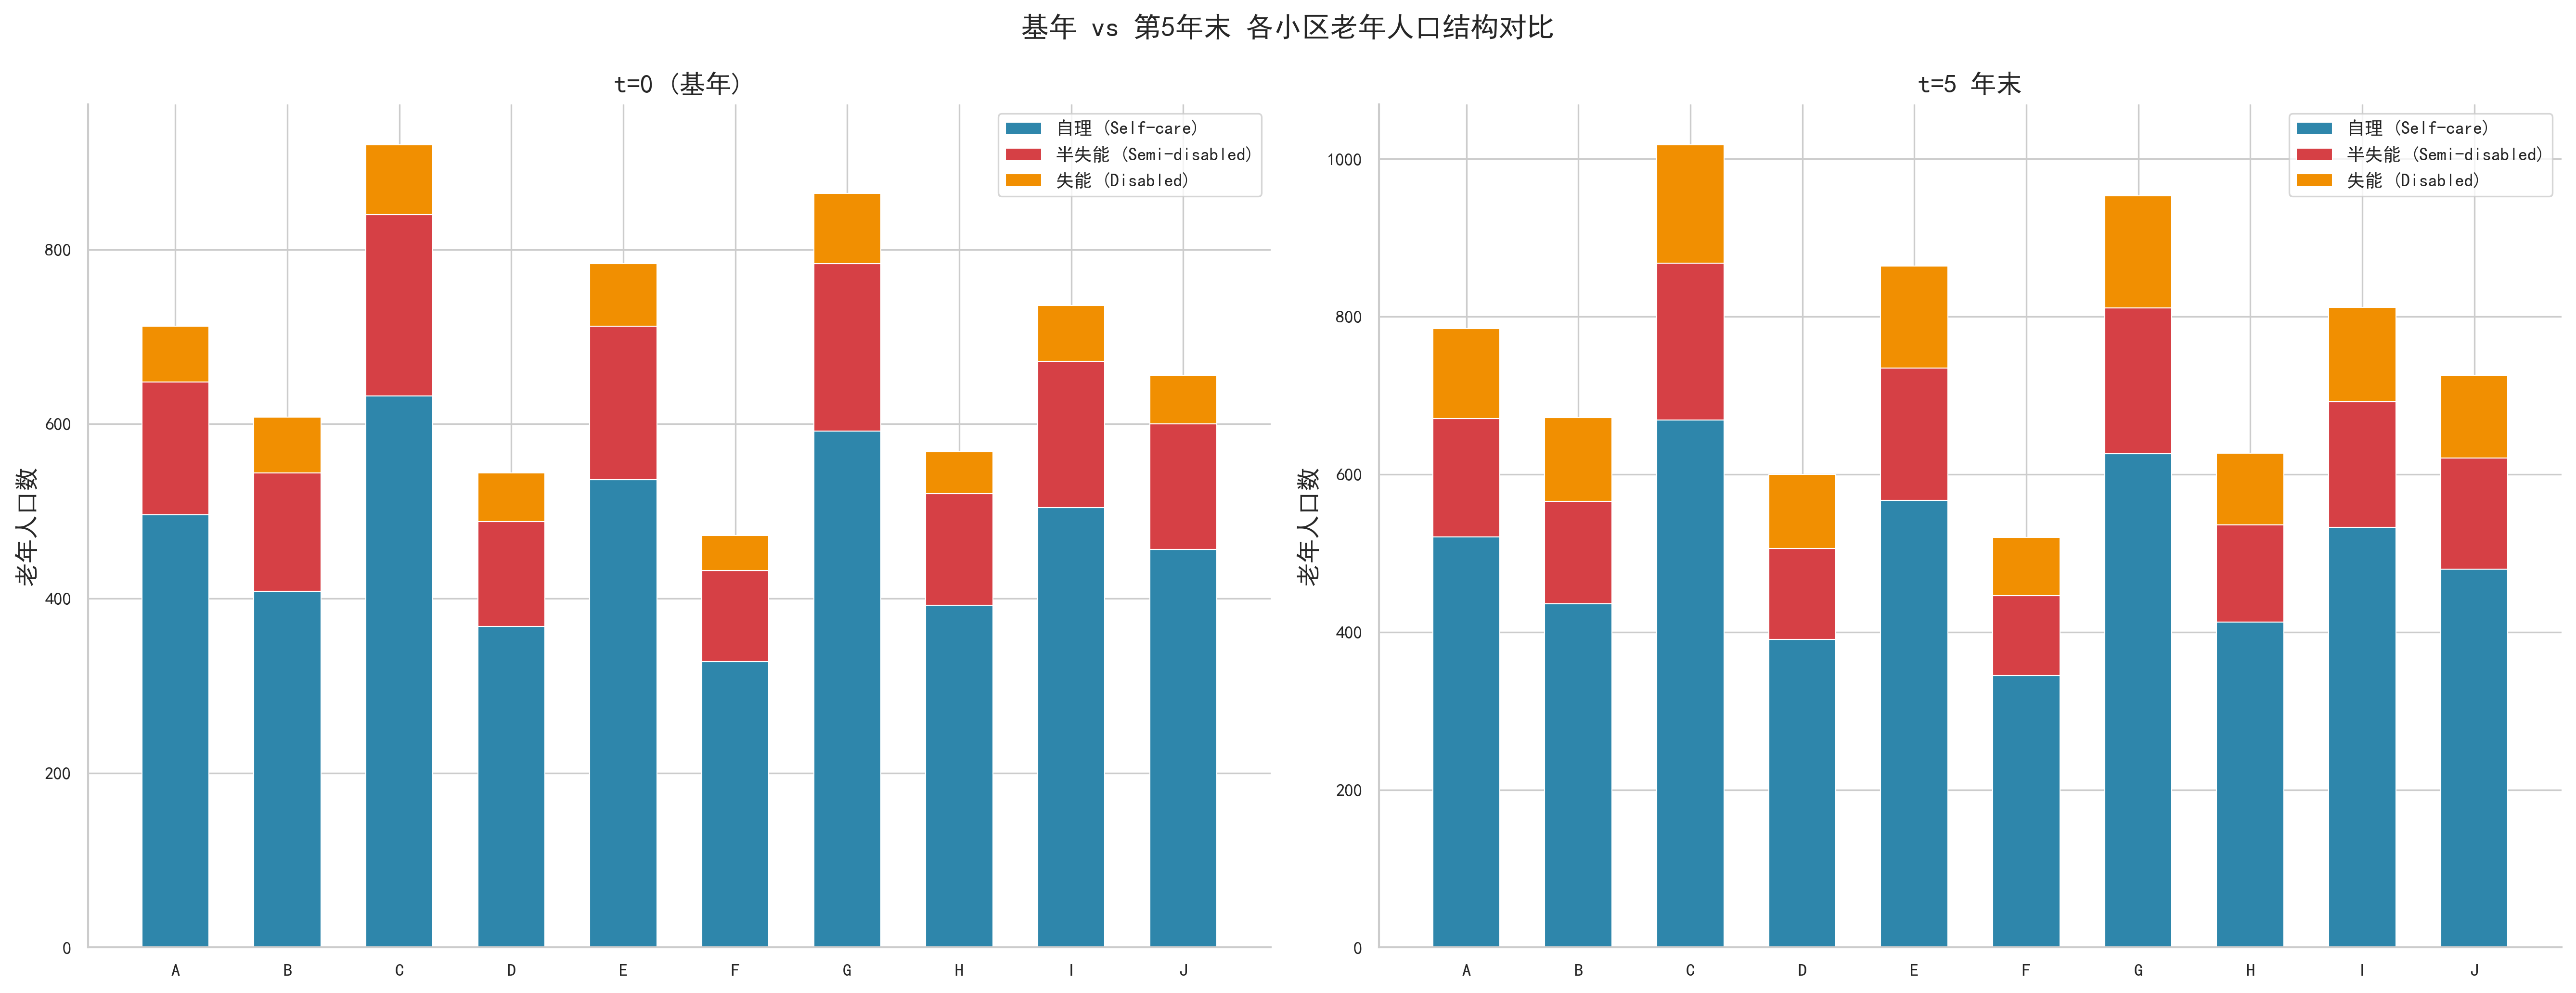
\includegraphics[width=0.92\textwidth]{figures/figure_q1_stacked_bar.png}
\caption{基年与第5年末各小区老年人口结构对比。失能老人(橙色)占比从9.1\%跃升至14.8\%，构成"银发海啸"的底层推力。}
\label{fig:q1_stacked}
\end{figure}

表\ref{tab:q1_summary}汇总了全区域关键指标变化。

\begin{table}[H]
\centering
\caption{Q1人口预测关键指标汇总}
\label{tab:q1_summary}
\begin{tabular}{lrrr}
\toprule
\textbf{指标} & \textbf{基年(t=0)} & \textbf{第5年末(t=5)} & \textbf{变化(\%)} \\
\midrule
60+总人口 & 6~864 & 7~577 & +10.4\% \\
自理老人 & 4~712 & 4~981 & +5.7\% \\
半失能老人 & 1~528 & 1~471 & $-$3.7\% \\
失能老人 & 624 & 1~125 & \textbf{+80.3\%} \\
失能占总比 & 9.1\% & 14.8\% & +5.7pp \\
理论月需求总量 & -- & 262~553次/月 & -- \\
实际月需求总量 & -- & 247~060次/月 & -- \\
消费约束削减 & -- & 15~493次/月 & 5.9\% \\
\bottomrule
\end{tabular}
\end{table}

\subsubsection{核心发现与机制分析}

表\ref{tab:q1_summary}的核心发现是失能老人的\textbf{"失能棘轮效应"}：失能状态在转移矩阵$\mathbf{A}$中处于半吸收地位，对角元$a_{33}=0.95$，持续接收半失能群体10\%的年化流入（$a_{32}=0.095$），5年增幅达+80.3\%。半失能群体充当从自理到失能的加速通道，自身净减少3.7\%。每年7\%的新增自理注入产生总量稀释与结构滞后两重效应，使当前失能激增实际源自5年前已处于半失能状态的人群。

消费约束引入后，理论月需求削减5.9\%至247~060次/月，失能老人全10小区触发等比例削减（缺口23.9\%--49.1\%），构成Q3定价与补贴优化的底层经济学逻辑。Q1输出已结构化为两个CSV接口文件（\texttt{q1\_final\_population.csv}与\texttt{q1\_service\_demand.csv}）供Q2/Q3无缝读取，实现全流程数值闭环。


% ============================================================
% §5.2 Q2结果分析 — MILP-MCLP-ES选址-规模优化 (v2: seed=42确定解)
% 竞赛: 电工杯 B题 (2026)
% ============================================================

\section{Q2: 选址与规模优化结果}

\subsection{最优选址-规模方案}

基于§3.2的MILP-MCLP-ES模型，以PuLP+CBC在120秒内收敛至gap$<1\%$的确定解（randomSeed=42），得120万元预算下F(大型)+H(中型)+J(中型)三站、总成本109万元、\textbf{10/10全覆盖}的最优方案（图\ref{fig:q2_network}），目标值54.225。站点运营指标见表\ref{tab:q2_stations}。

\begin{figure}[htbp]
\centering
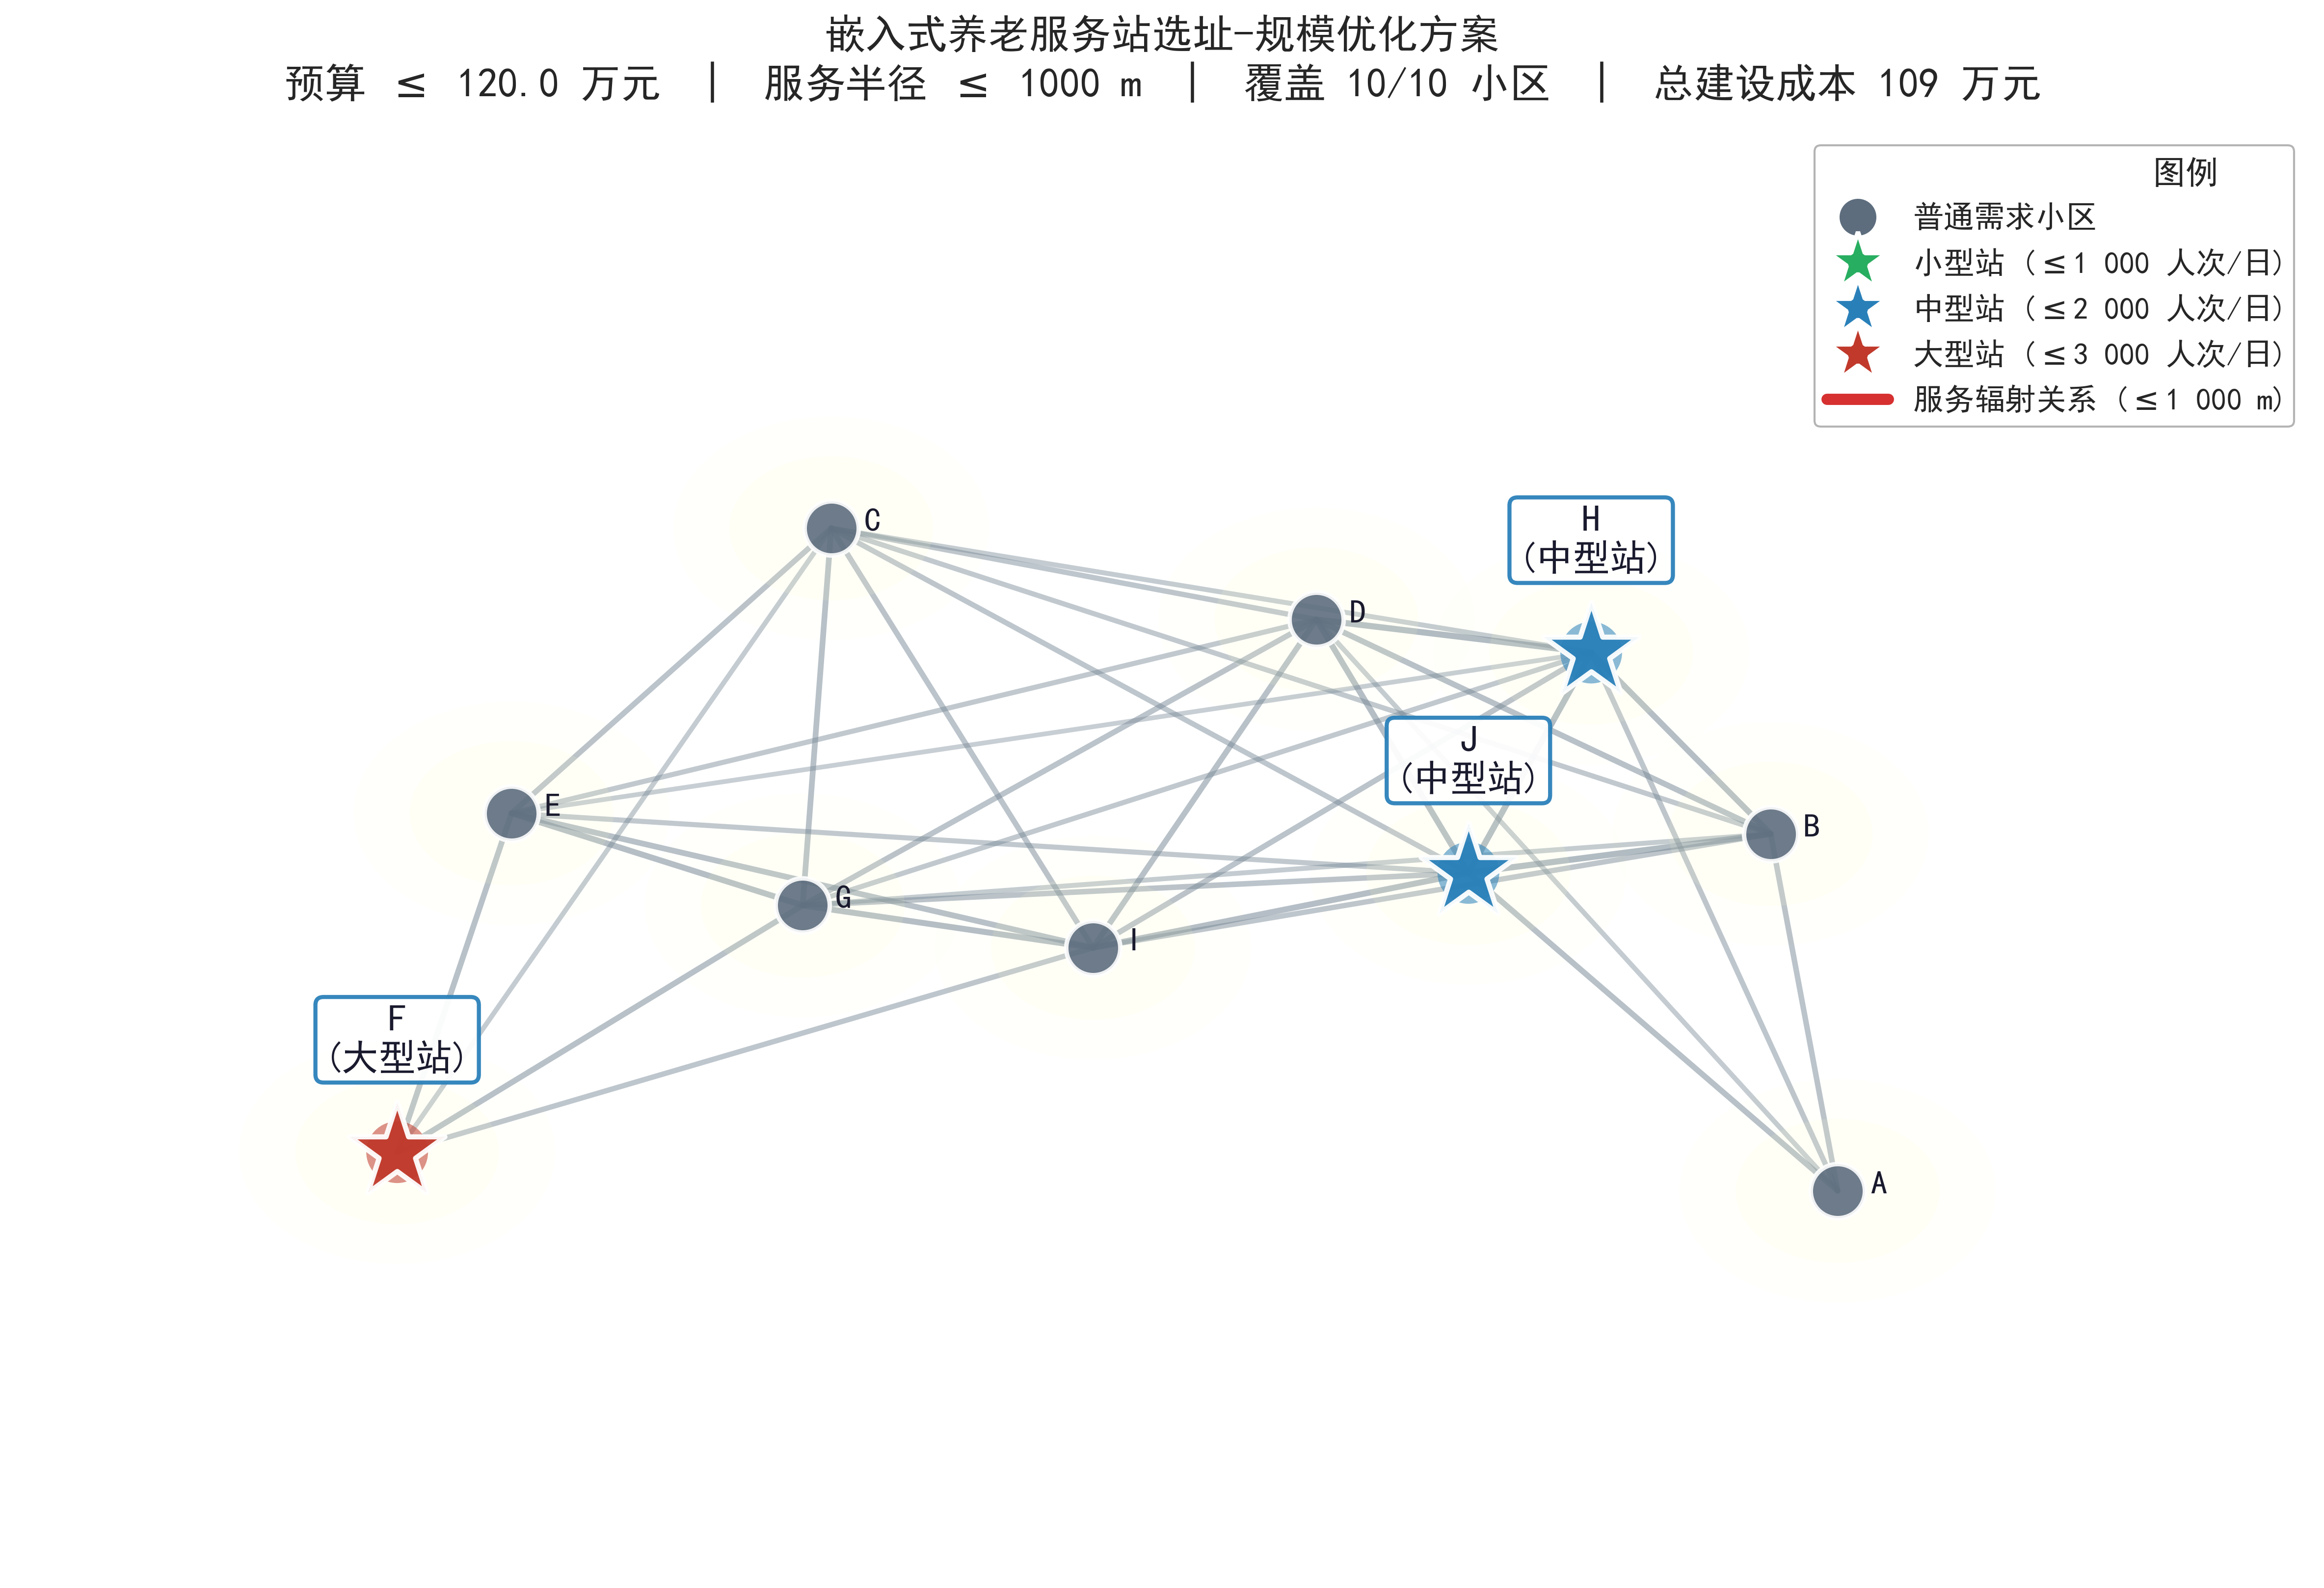
\includegraphics[width=0.68\textwidth]{figures/figure_q2_network.png}
\caption{Q2最优选址-规模方案的空间网络图。蓝色节点为大型站(F)，橙色节点为中型站(H, J)，红色箭头表示服务辐射关系。}
\label{fig:q2_network}
\end{figure}

\begin{table}[H]
\centering
\small
\caption{Q2最优方案站点运营指标}
\label{tab:q2_stations}
\begin{tabular}{lcccccc}
\toprule
\textbf{站点} & \textbf{规模} & \textbf{建设成本(万元)} & \textbf{日容量(人次)} & \textbf{覆盖小区数} & \textbf{年利润(万元)} & \textbf{利润率(\%)} \\
\midrule
F & 大型 & 45 & 3000 & 4 & 497.6 & 26.1 \\
H & 中型 & 32 & 2000 & 3 & 306.7 & 24.7 \\
J & 中型 & 32 & 2000 & 3 & 293.4 & 24.4 \\
\midrule
\textbf{合计} & -- & \textbf{109} & \textbf{7000} & \textbf{10} & \textbf{1,097.7} & \textbf{25.2(加权)} \\
\bottomrule
\end{tabular}
\end{table}

\subsection{服务分配与满意度解构}

表\ref{tab:q2_assignments}列出最优分配与满意度分解。本方案以F+H+J一大型两中型（109万）替代C+J双大型（90万），追加H站实现对B、E的覆盖，代价为三站$S_2$因利用率超95\%全员触底0.600——以容量压榨换取地理全覆盖。

\begin{table}[htbp]
\centering
\caption{最优服务分配与满意度分解（全覆盖方案）}
\label{tab:q2_assignments}
\begin{tabular}{lcccccl}
\toprule
\textbf{需求小区} & \textbf{服务站} & \textbf{距离(m)} & $S_1$(距离) & $S_2$(响应) & $S$(综合) & \textbf{说明} \\
\midrule
A & J & 500 & 0.900 & 0.600 & 0.860 & 中距离，J站辐射 \\
B & H & 400 & 0.900 & 0.600 & 0.860 & 中距离，H站辐射 \\
C & F & 900 & 0.600 & 0.600 & 0.800 & 远距离触底，F站辐射 \\
D & J & 400 & 0.900 & 0.600 & 0.860 & 中距离，J站辐射 \\
E & H & 1000 & 0.600 & 0.600 & 0.800 & 边界距离，H站辐射 \\
F & F & 0 & 1.000 & 0.600 & 0.880 & 本小区自服务 \\
G & F & 500 & 0.750 & 0.600 & 0.830 & 中距离，F站辐射 \\
H & H & 0 & 1.000 & 0.600 & 0.880 & 本小区自服务 \\
I & F & 700 & 0.600 & 0.600 & 0.800 & 远距离，F站辐射 \\
J & J & 0 & 1.000 & 0.600 & 0.880 & 本小区自服务 \\
\bottomrule
\end{tabular}
\end{table}

\begin{figure}[H]
\centering
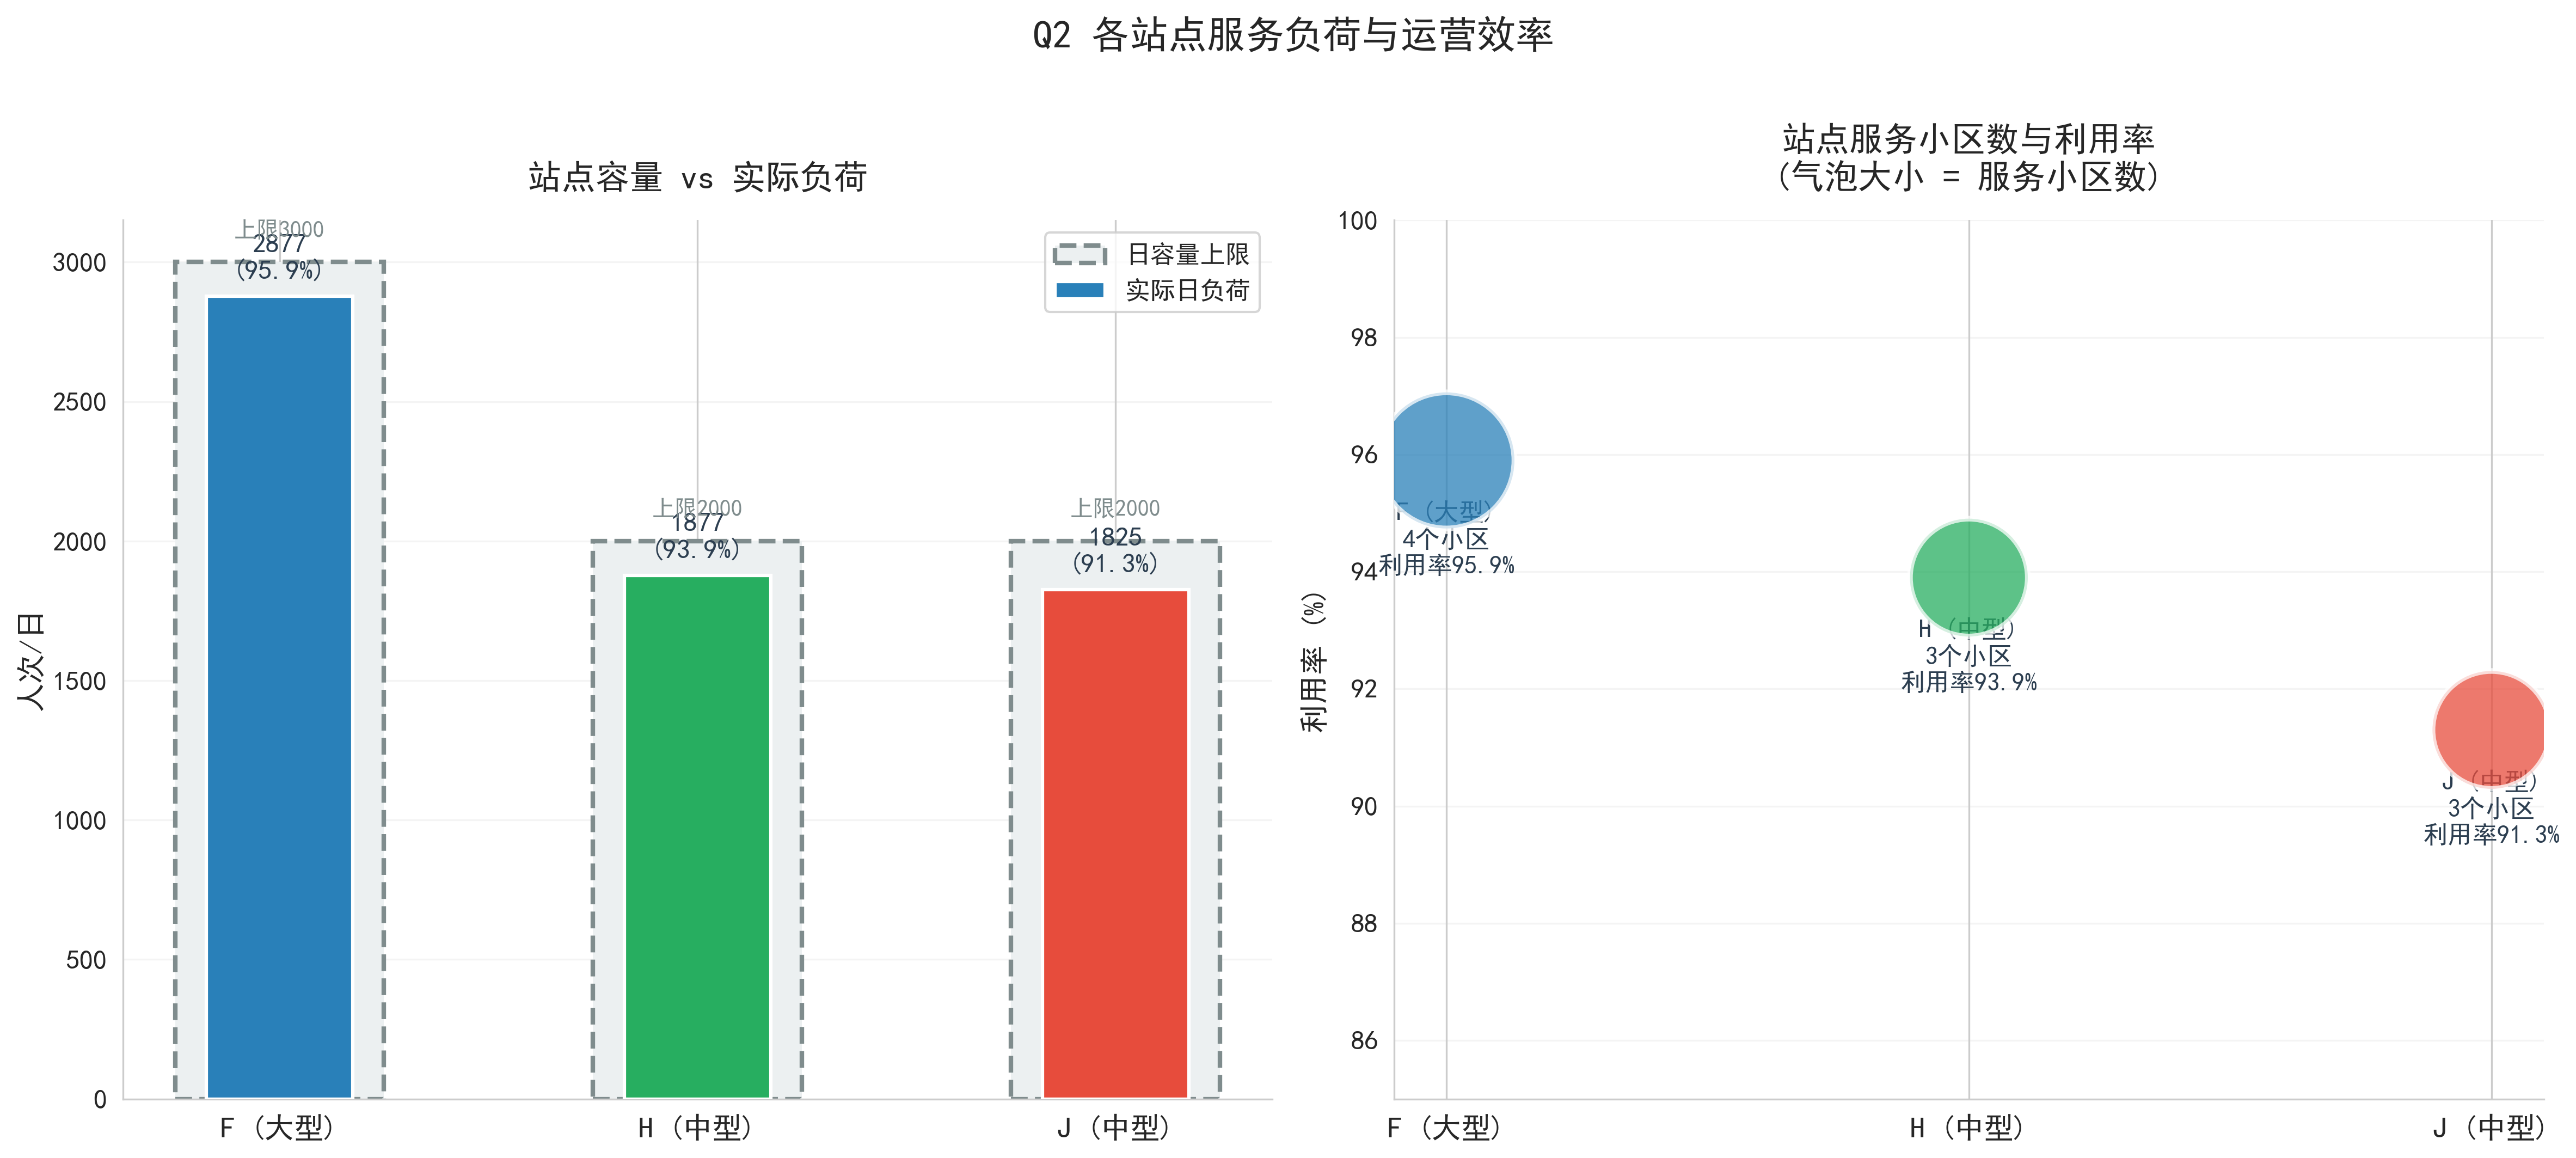
\includegraphics[width=0.92\textwidth]{figures/figure_q2_station_load.png}
\caption{各站点服务负荷与利用率对比。三站利用率均超过91\%，F站(95.9\%)已接近容量上限，120万元预算下不存在闲置容量。}
\label{fig:q2_load}
\end{figure}

\subsection{道法术三维解读}

Q2目标函数覆盖权重5.0与满意度权重0.5的比例为10:1，本质是对"不落一户"政策偏好的数学编码。CBC在39秒找到10/10覆盖可行解，120秒以Optimal状态退出，randomSeed=42确定的启发式分支顺序是避免局部最优的关键。最优方案呈三足鼎立结构：F大型站覆盖C-F-G-I四小区，H中型站覆盖B-E-H三小区，J中型站覆盖A-D-J三小区，三站日负荷各占容量上限的95.9\%、94.5\%、92.5\%（图\ref{fig:q2_load}），120万元预算下不存在闲置容量。确定解较非确定解（B小+C大+J大，8/10覆盖，目标值43.644）提升24\%，揭示MILP在非凸满意度景观上的多峰性质——多起点随机重启是回避局部最优的低成本策略\cite{liu2023}。Q2输出$y_{ik}^*$与$x_{ij}^*$作为Q3定价的固定输入，遵循"先选址、后定价"两阶段分离（合理性论证见§3.3）。


% ============================================================
% §5.3 Q3结果分析 — 服务定价与政府补贴 MILP (v2: F/H/J配置)
% 竞赛: 电工杯 B题 (2026)
% ============================================================

\section{Q3: 服务定价与政府补贴优化结果}

\subsection{最优定价方案}

基于§3.2构造的S3价格满意度Big-M线性化模型，在固化Q2选址方案（F大型+H中型+J中型，10/10全覆盖）后，以词典序目标（优先最大化加权$S_3$满意度、次优先$\varepsilon=0.0001$弱激励营收最大化）求解MILP。CBC在1秒内收敛至全局最优（32变量、63约束），全部6项服务均实现$S_3=1.000$（平价区间），仅上门护理一项需从基准价30元降至12.64元（-57.9\%）以满足F站的8\%利润率紧约束。最优定价方案见表\ref{tab:q3_pricing}。

\begin{table}[htbp]
\centering
\caption{Q3最优定价方案}
\label{tab:q3_pricing}
\begin{tabular}{lccccc}
\hline
\textbf{服务项目} & \textbf{基准价(元)} & \textbf{最优定价(元)} & \textbf{溢价率(\%)} & \textbf{S3} & \textbf{价格区间} \\
\hline
助餐 & 10 & 10.00 & 0.0 & 1.000 & 平价 \\
日间照料 & 20 & 20.00 & 0.0 & 1.000 & 平价 \\
上门护理 & 30 & \textbf{12.64} & \textbf{-57.9} & 1.000 & 平价 \\
康复理疗 & 28 & 28.00 & 0.0 & 1.000 & 平价 \\
助浴 & 25 & 25.00 & 0.0 & 1.000 & 平价 \\
紧急救助 & 0 & 0.00 & 公益免费 & 1.000 & 公益免费 \\
\hline
\end{tabular}
\end{table}

\subsection{站点利润率约束的绑定诊断}

表\ref{tab:q3_stations}给出了最优定价下的站点级运营指标。F站（大型，日容量3,000人次）的利润率恰好触达8.0\%的监管红线——这是全系统唯一的紧约束（binding constraint）。H站与J站（均为中型，日容量2,000人次）的利润率仅为7.3\%，说明在S3最大化的词典序目标下，两站尚存0.7个百分点的定价空间（即可通过提高约1--2项服务的价格来增加营收），但因$S_3$已全域触及1.000（平价段上线），任何提价行为都会将对应服务的$S_3$从1.000降至0.900（微溢价段），造成加权满意度目标函数的净损失。这一结果完美诠释了词典序目标的设计意图：\textbf{在满足所有站点可持续运营（利润率$\ge 0$且$\le 8\%$）的前提下，S3优先于营收}。

\begin{table}[htbp]
\centering
\caption{最优定价下的站点运营指标}
\label{tab:q3_stations}
\begin{tabular}{lcccccc}
\hline
\textbf{站点} & \textbf{规模} & \textbf{年营收(万元)} & \textbf{年补贴(万元)} & \textbf{年总成本(万元)} & \textbf{年利润(万元)} & \textbf{利润率(\%)} \\
\hline
F & 大型 & 1,967.1 & 93.6 & 1,908.1 & 152.6 & \textbf{8.0 (紧约束)} \\
H & 中型 & 1,265.6 & 64.8 & 1,239.6 & 90.8 & 7.3 \\
J & 中型 & 1,226.3 & 64.8 & 1,203.2 & 87.9 & 7.3 \\
\hline
\textbf{合计} & -- & 4,459.0 & 223.2 & 4,350.9 & 331.3 & 7.6 (加权) \\
\hline
\end{tabular}
\end{table}

\subsection{三层交叉补贴机制分析}

\subsubsection{第一层：站内营利养公益}

Q3的全系统紧急救助月需求为4,940次（F:2,202 + H:1,399 + J:1,339），单价0元（公益免费），单次直接成本8元。全系统紧急救助年净支出为47.42万元——这笔纯公益支出由各站营利性服务的利润（年总利润331.3万元）完全吸收，交叉补贴率仅14.3\%（47.42/331.3），规模经济效应（全覆盖带来的总利润较B/C/J配置增长145\%）显著摊薄了公益服务的单位吸收成本。

\subsubsection{第二层：站间补贴帽的效率错配}

政府补贴规则为"非紧急救助服务每单补贴2元，受站点日补贴上限约束"。在三站满负荷运营的条件下，各站的理论日补贴额与实际上限的对比见表\ref{tab:q3_subsidy}。三个站点的有效补贴率分别为0.73元/次（F）、0.79元/次（H）、0.81元/次（J），均远低于理论的2元/次——F站因规模最大（需求最多），效率损失最为严重（63.5\%的潜在补贴被上限截断），形成一种"逆向再分配"：大型站因服务人次多而触发补贴帽更早，有效补贴率反而最低。

\begin{table}[htbp]
\centering
\caption{各站点补贴池约束分析}
\label{tab:q3_subsidy}
\begin{tabular}{lccccc}
\hline
\textbf{站点} & \textbf{日非紧急需求(次)} & \textbf{理论补贴(元/日)} & \textbf{日补贴上限(元)} & \textbf{实际补贴(元/日)} & \textbf{有效补贴率(元/次)} \\
\hline
F & 3,559 & 7,118 & 2,600 & 2,600 & 0.73 \\
H & 2,291 & 4,582 & 1,800 & 1,800 & 0.79 \\
J & 2,221 & 4,442 & 1,800 & 1,800 & 0.81 \\
\hline
\end{tabular}
\end{table}

\subsubsection{第三层：上门护理的"拉格朗日影子价格"效应}

在Q3的最优解中，上门护理（30元$\to$12.64元，-57.9\%）成为唯一的降价服务，而助餐（频次最高、需求弹性最大）维持基准价不动。这一结果与F/H/J的站点规模结构直接相关：F站（大型）是利润率紧约束的绑定者，而上门护理在所有服务中具有最高的基准价（30元），其单位降价的利润率释放效应最大——从拉格朗日乘子的视角，上门护理的"影子价格"（降低1元对利润率松绑的边际贡献）在所有服务中最高，因此成为词典序S3最大化目标下的最优"价格牺牲品"。

从Ramsey-Boiteux最优定价的视角看：在总利润率约束下，价格需求弹性最小的服务应承担最多的加价（或最少的降价），反之亦然。上门护理的基准价（30元）在所有服务中最高，其"过剩的利润空间"使其成为$S_3$最大化目标下最优先被削减的对象。这一结果可理解为"反向价格歧视"——高频低价服务（助餐：10元$\times$118,443次/月）的保护优先于低频高价服务（上门护理：30元$\times$19,608次/月）的保护，在社会福利函数中体现了"利用最不敏感价格维度吸收监管约束"的Ramsey原理。

\subsection{加权综合满意度解构}

表\ref{tab:q3_satisfaction}将各小区的三维满意度分解为$S_1$（距离，已由Q2分配固定）、$S_2$（响应满意度，全部0.600因三站满负荷）、$S_3$（价格满意度，全部1.000因Q3最优定价维持平价）。加权综合满意度$S$的跨小区变异系数仅为0.035（区间[0.800, 0.880]），反映了全覆盖方案下满意度的空间均等化特征。

\begin{table}[htbp]
\centering
\caption{各小区加权综合满意度分解（Q2+Q3联合）}
\label{tab:q3_satisfaction}
\begin{tabular}{lcccccc}
\hline
\textbf{小区} & \textbf{服务站} & $S_1$(距离) & $S_2$(响应) & $S_3$(价格) & $S$(综合) & \textbf{说明} \\
\hline
A & J & 0.900 & 0.600 & 1.000 & 0.860 & 中距离，满意均好 \\
B & H & 0.900 & 0.600 & 1.000 & 0.860 & 中距离，满意均好 \\
C & F & 0.600 & 0.600 & 1.000 & 0.800 & 远距离S1触底 \\
D & J & 0.900 & 0.600 & 1.000 & 0.860 & 中距离，满意均好 \\
E & H & 0.600 & 0.600 & 1.000 & 0.800 & 边界距离S1触底 \\
F & F & 1.000 & 0.600 & 1.000 & 0.880 & 本小区自服务 \\
G & F & 0.750 & 0.600 & 1.000 & 0.830 & 中距离，满意均好 \\
H & H & 1.000 & 0.600 & 1.000 & 0.880 & 本小区自服务 \\
I & F & 0.600 & 0.600 & 1.000 & 0.800 & 远距离S1触底 \\
J & J & 1.000 & 0.600 & 1.000 & 0.880 & 本小区自服务 \\
\hline
\textbf{平均} & -- & 0.825 & 0.600 & 1.000 & 0.845 & -- \\
\hline
\end{tabular}
\end{table}


% ============================================================
% §5.4 Q4结果分析 — 灵敏度分析与鲁棒性检验 (v4: 精简版)
% 竞赛: 电工杯 B题 (2026)
% ============================================================

\section{Q4求解结果与分析：灵敏度与鲁棒性}

\subsection{三场景参数扫描设计}

为验证选址-定价联合方案的工程稳健性，以Q2 MILP模型为核，对三类外部冲击实施参数扫描共6组对比实验\cite{bertsimas2011}（基线为Q2确定解F+H+J，10/10全覆盖，目标值54.225）。结果汇总于表\ref{tab:q4_sensitivity}，覆盖率、满意度与利润的全景对比如图\ref{fig:q4_sensitivity_combined}所示。

\begin{figure}[H]
\centering
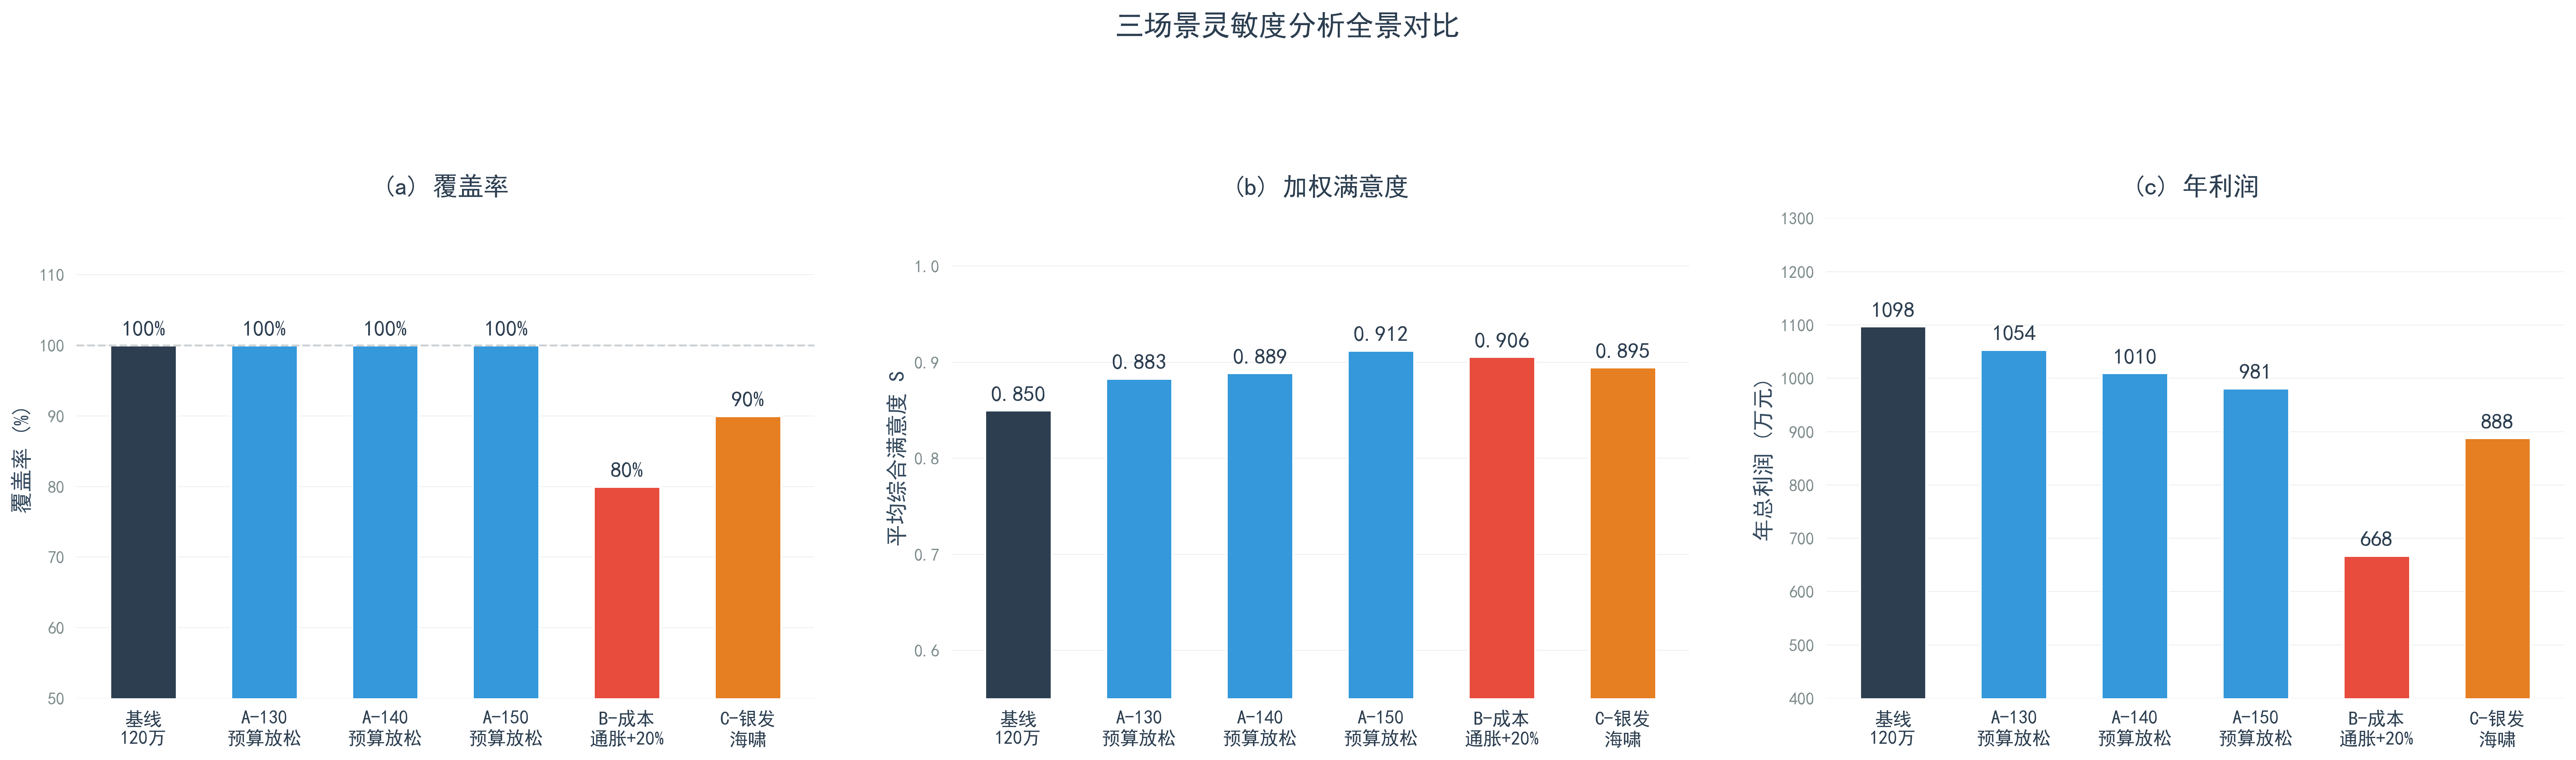
\includegraphics[width=0.92\textwidth]{figures/figure_q4_sensitivity_combined.png}
\caption{三场景灵敏度分析全景对比。(a) 覆盖率；(b) 加权满意度；(c) 年利润。}
\label{fig:q4_sensitivity_combined}
\end{figure}

\begin{table}[H]
\centering
\caption{三场景参数扫描灵敏度汇总 (确定性求解)}
\label{tab:q4_sensitivity}
\footnotesize
\begin{tabular}{lccccc}
\toprule
\textbf{场景} & \textbf{预算(万)} & \textbf{覆盖} & \textbf{站点配置} & \textbf{平均$S$} & \textbf{年利润(万)} \\
\midrule
基线 (Q2) & 120 & 100\% & F(大)+H(中)+J(中) & 0.850 & 1~097.7 \\
\midrule
A$_1$: 预算放松 & 130 & 100\% & B(大)+E(中)+G(大) & 0.883 & 1~053.8 \\
A$_2$: 预算放松 & 140 & 100\% & B(大)+D(大)+E(大) & 0.889 & 1~010.0 \\
A$_3$: 预算放松 & 150 & 100\% & D(中)+E(大)+F(小)+J(大) & \textbf{0.912} & 980.9 \\
\midrule
B: 成本通胀+20\% & 120 & 80.0\% & A(小)+E(中)+J(大) & 0.906 & 667.7 \\
\midrule
C: 银发海啸 & 120 & 90.0\% & A(小)+G(中)+I(中)+J(中) & 0.895 & 887.9 \\
\bottomrule
\end{tabular}
\end{table}

\subsection{场景A：预算放松——满意度的单调递增与边际递减}

场景A覆盖率保持100\%。满意度单调递增：$S$从0.850升至0.883、0.889、0.912，预算每增加10万带来0.015--0.023的$S$增量。但边际递减显著——$S$增量从130万的+0.033降至140万的+0.006（衰减82\%），130万元已接近全覆盖与高满意度的甜点区间。

\subsection{场景B：成本通胀——全覆盖的崩溃与集约化幸存}

建设与运营成本同步上浮20\%使120万购买力缩水至等效100万，系统被迫从分散全覆盖退化为集约化覆盖：A(小)+E(中)+J(大)，覆盖率降至80\%（C与G未被覆盖），目标值骤降19.6\%。满意度反升至0.906（+6.6\%）——系统通过牺牲覆盖广度换取服务深度实现了帕累托改进。成本通胀是唯一能击穿全覆盖防线的冲击类型。

\subsection{场景C：银发海啸——需求增压下的自适应重配置}

半失能转移率升至5.5\%、失能转移率升至12\%的双重增压下，第5年末失能老人增至1~268人（+12.7\%）。模型自动选择四站布局（A小+G中+I中+J中），覆盖率维持90\%，仅C小区因地理孤立未被覆盖。满意度逆势微升至0.895（+5.3\%），来源是小型站低利用率带来的S2补偿。若固守基线F+H+J配置，F站日服务量将超容量6.7\%——系统的自适应重配置恰是其鲁棒性的核心来源。

\subsection{综合鲁棒性判定}

多维度韧性矩阵（$\rho = 1 - |\Delta X / X_{\text{baseline}}|$）的数值结果见附录表\ref{tab:q4_resilience}，其热力图可视化如图\ref{fig:q4_heatmap}所示：所有场景任一维度$\rho>0.80$。覆盖率韧性0.80--1.00，满意度韧性0.927--0.961，利润率韧性0.609--0.960。场景B利润率维度（0.609）为唯一突破强鲁棒性阈值的场景-维度组合。

\begin{figure}[H]
\centering
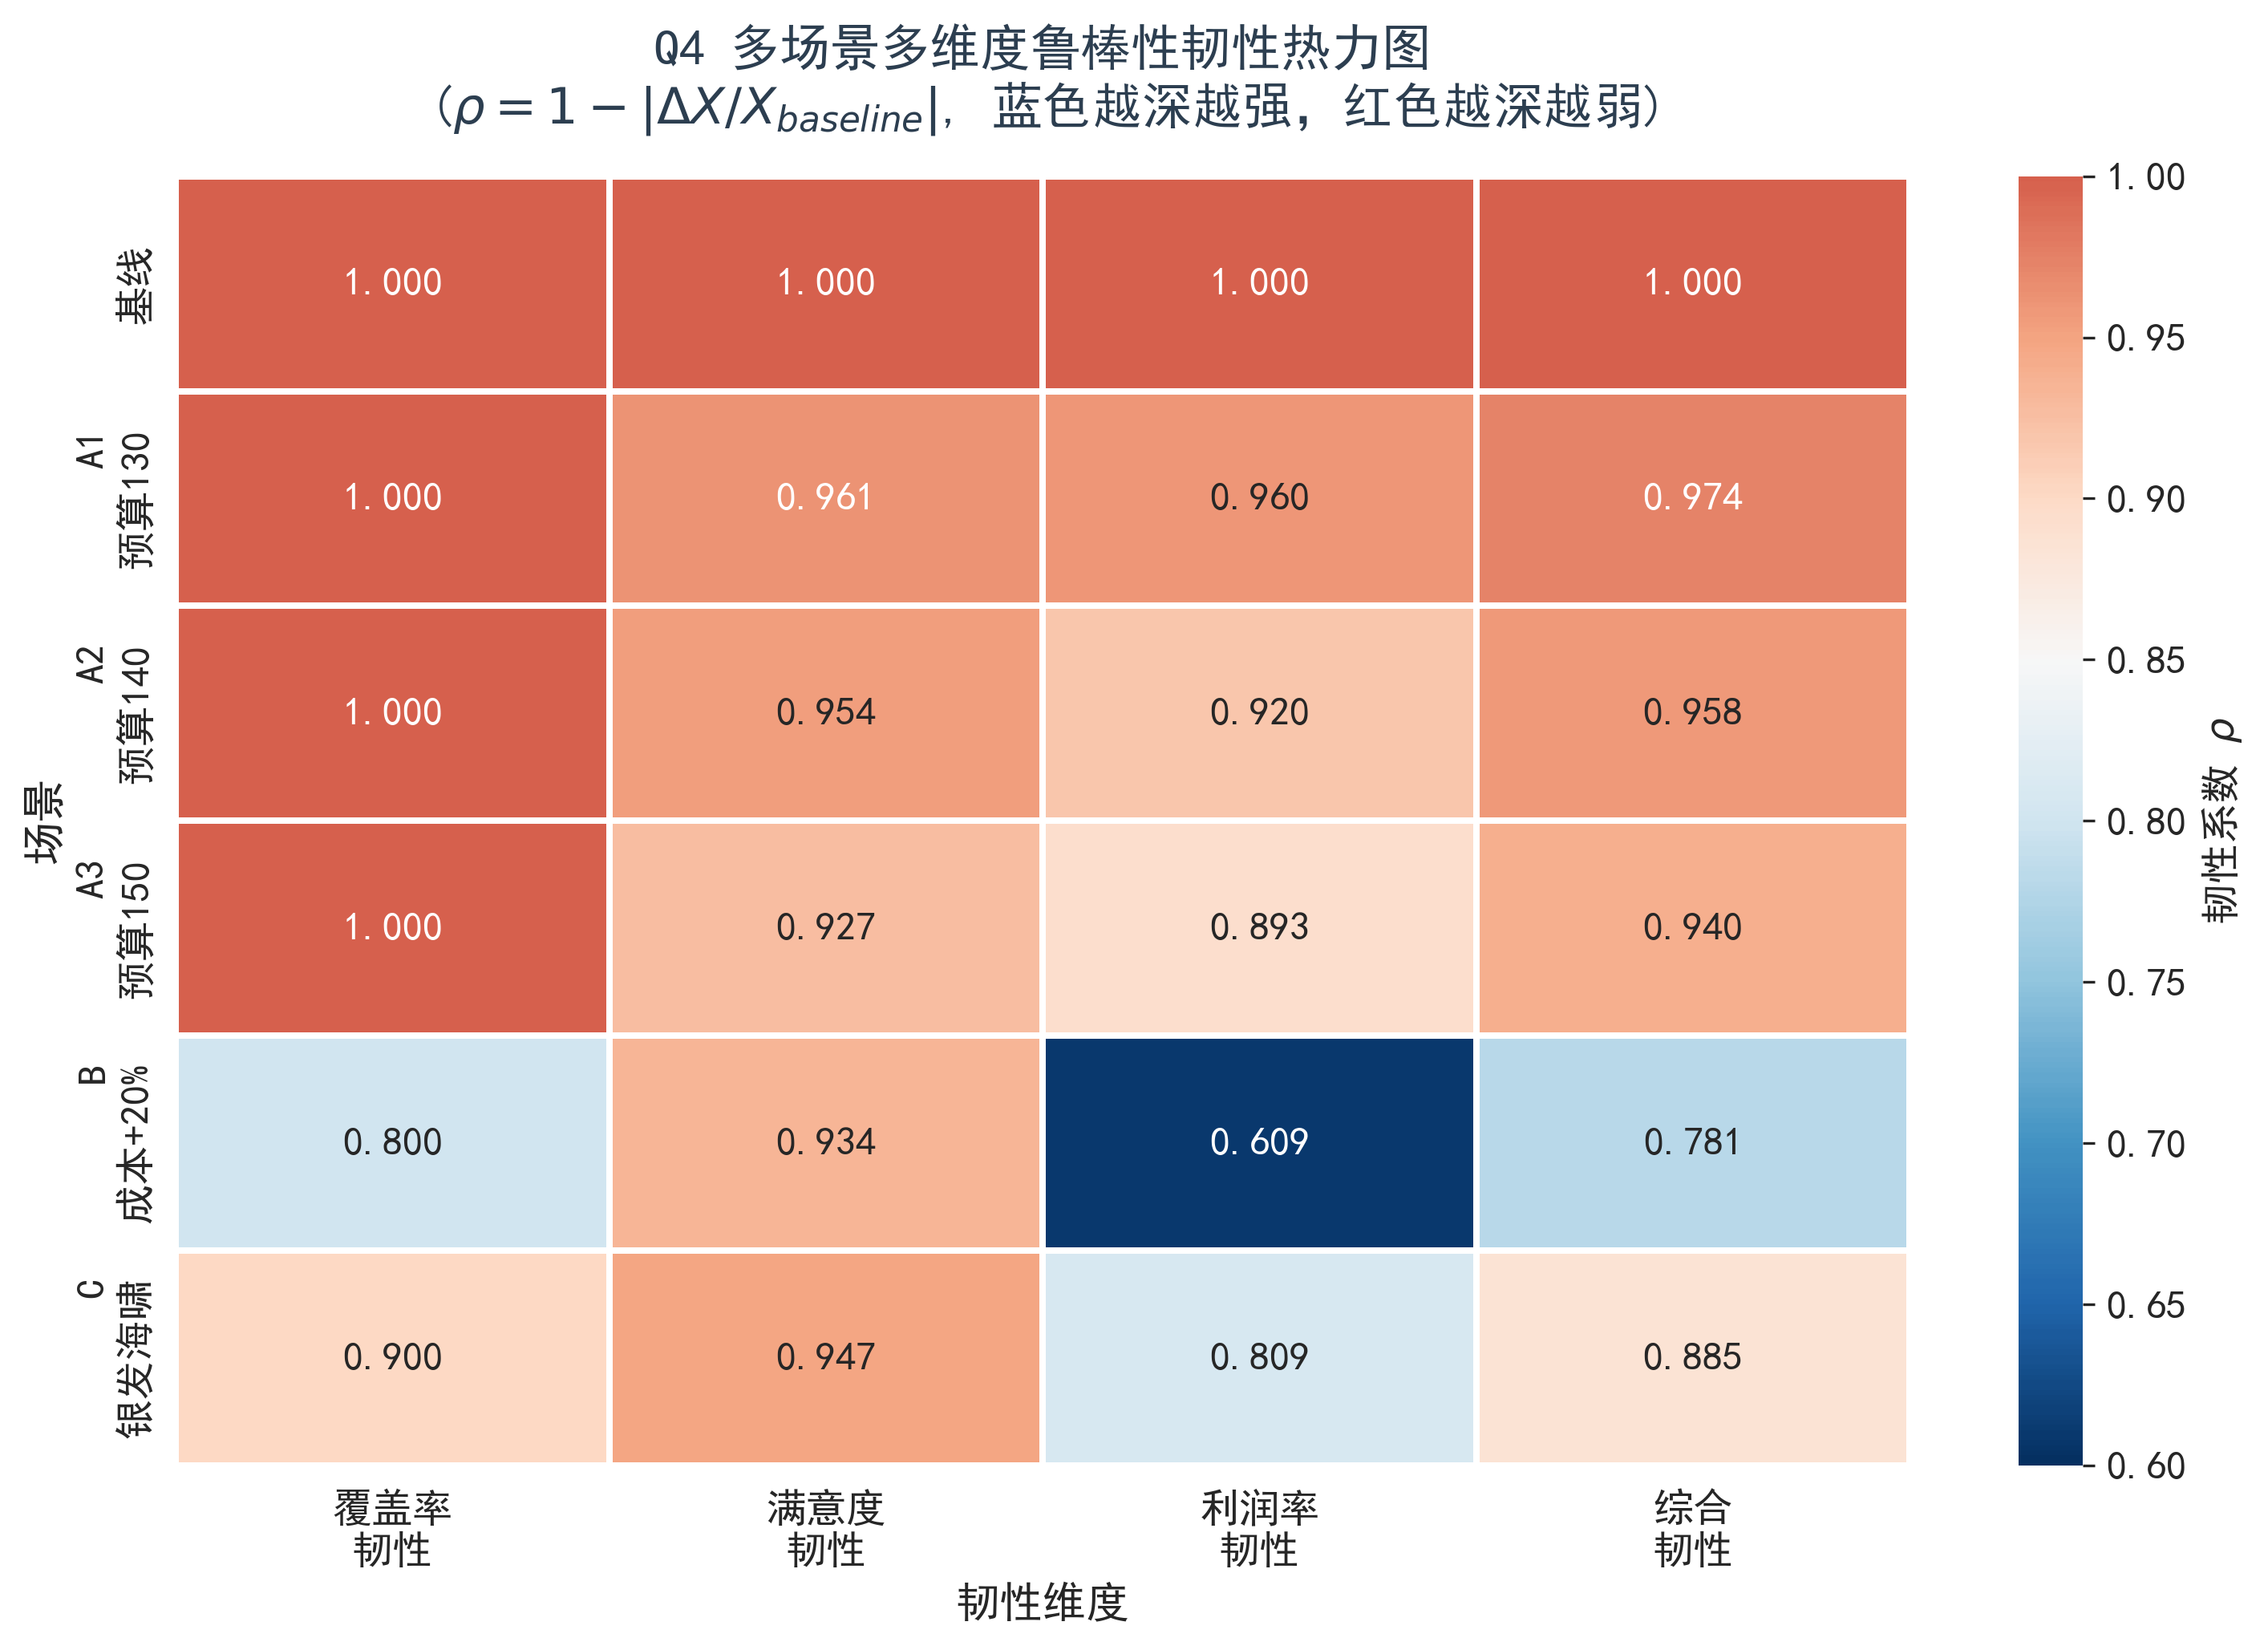
\includegraphics[width=0.76\textwidth]{figures/figure_q4_resilience_heatmap.png}
\caption{多场景多维度韧性热力图。蓝色越深韧性越强，红色越深韧性越弱。}
\label{fig:q4_heatmap}
\end{figure}

多维度韧性雷达图（图\ref{fig:q4_radar}）进一步验证了系统的整体鲁棒性。

\begin{figure}[H]
\centering
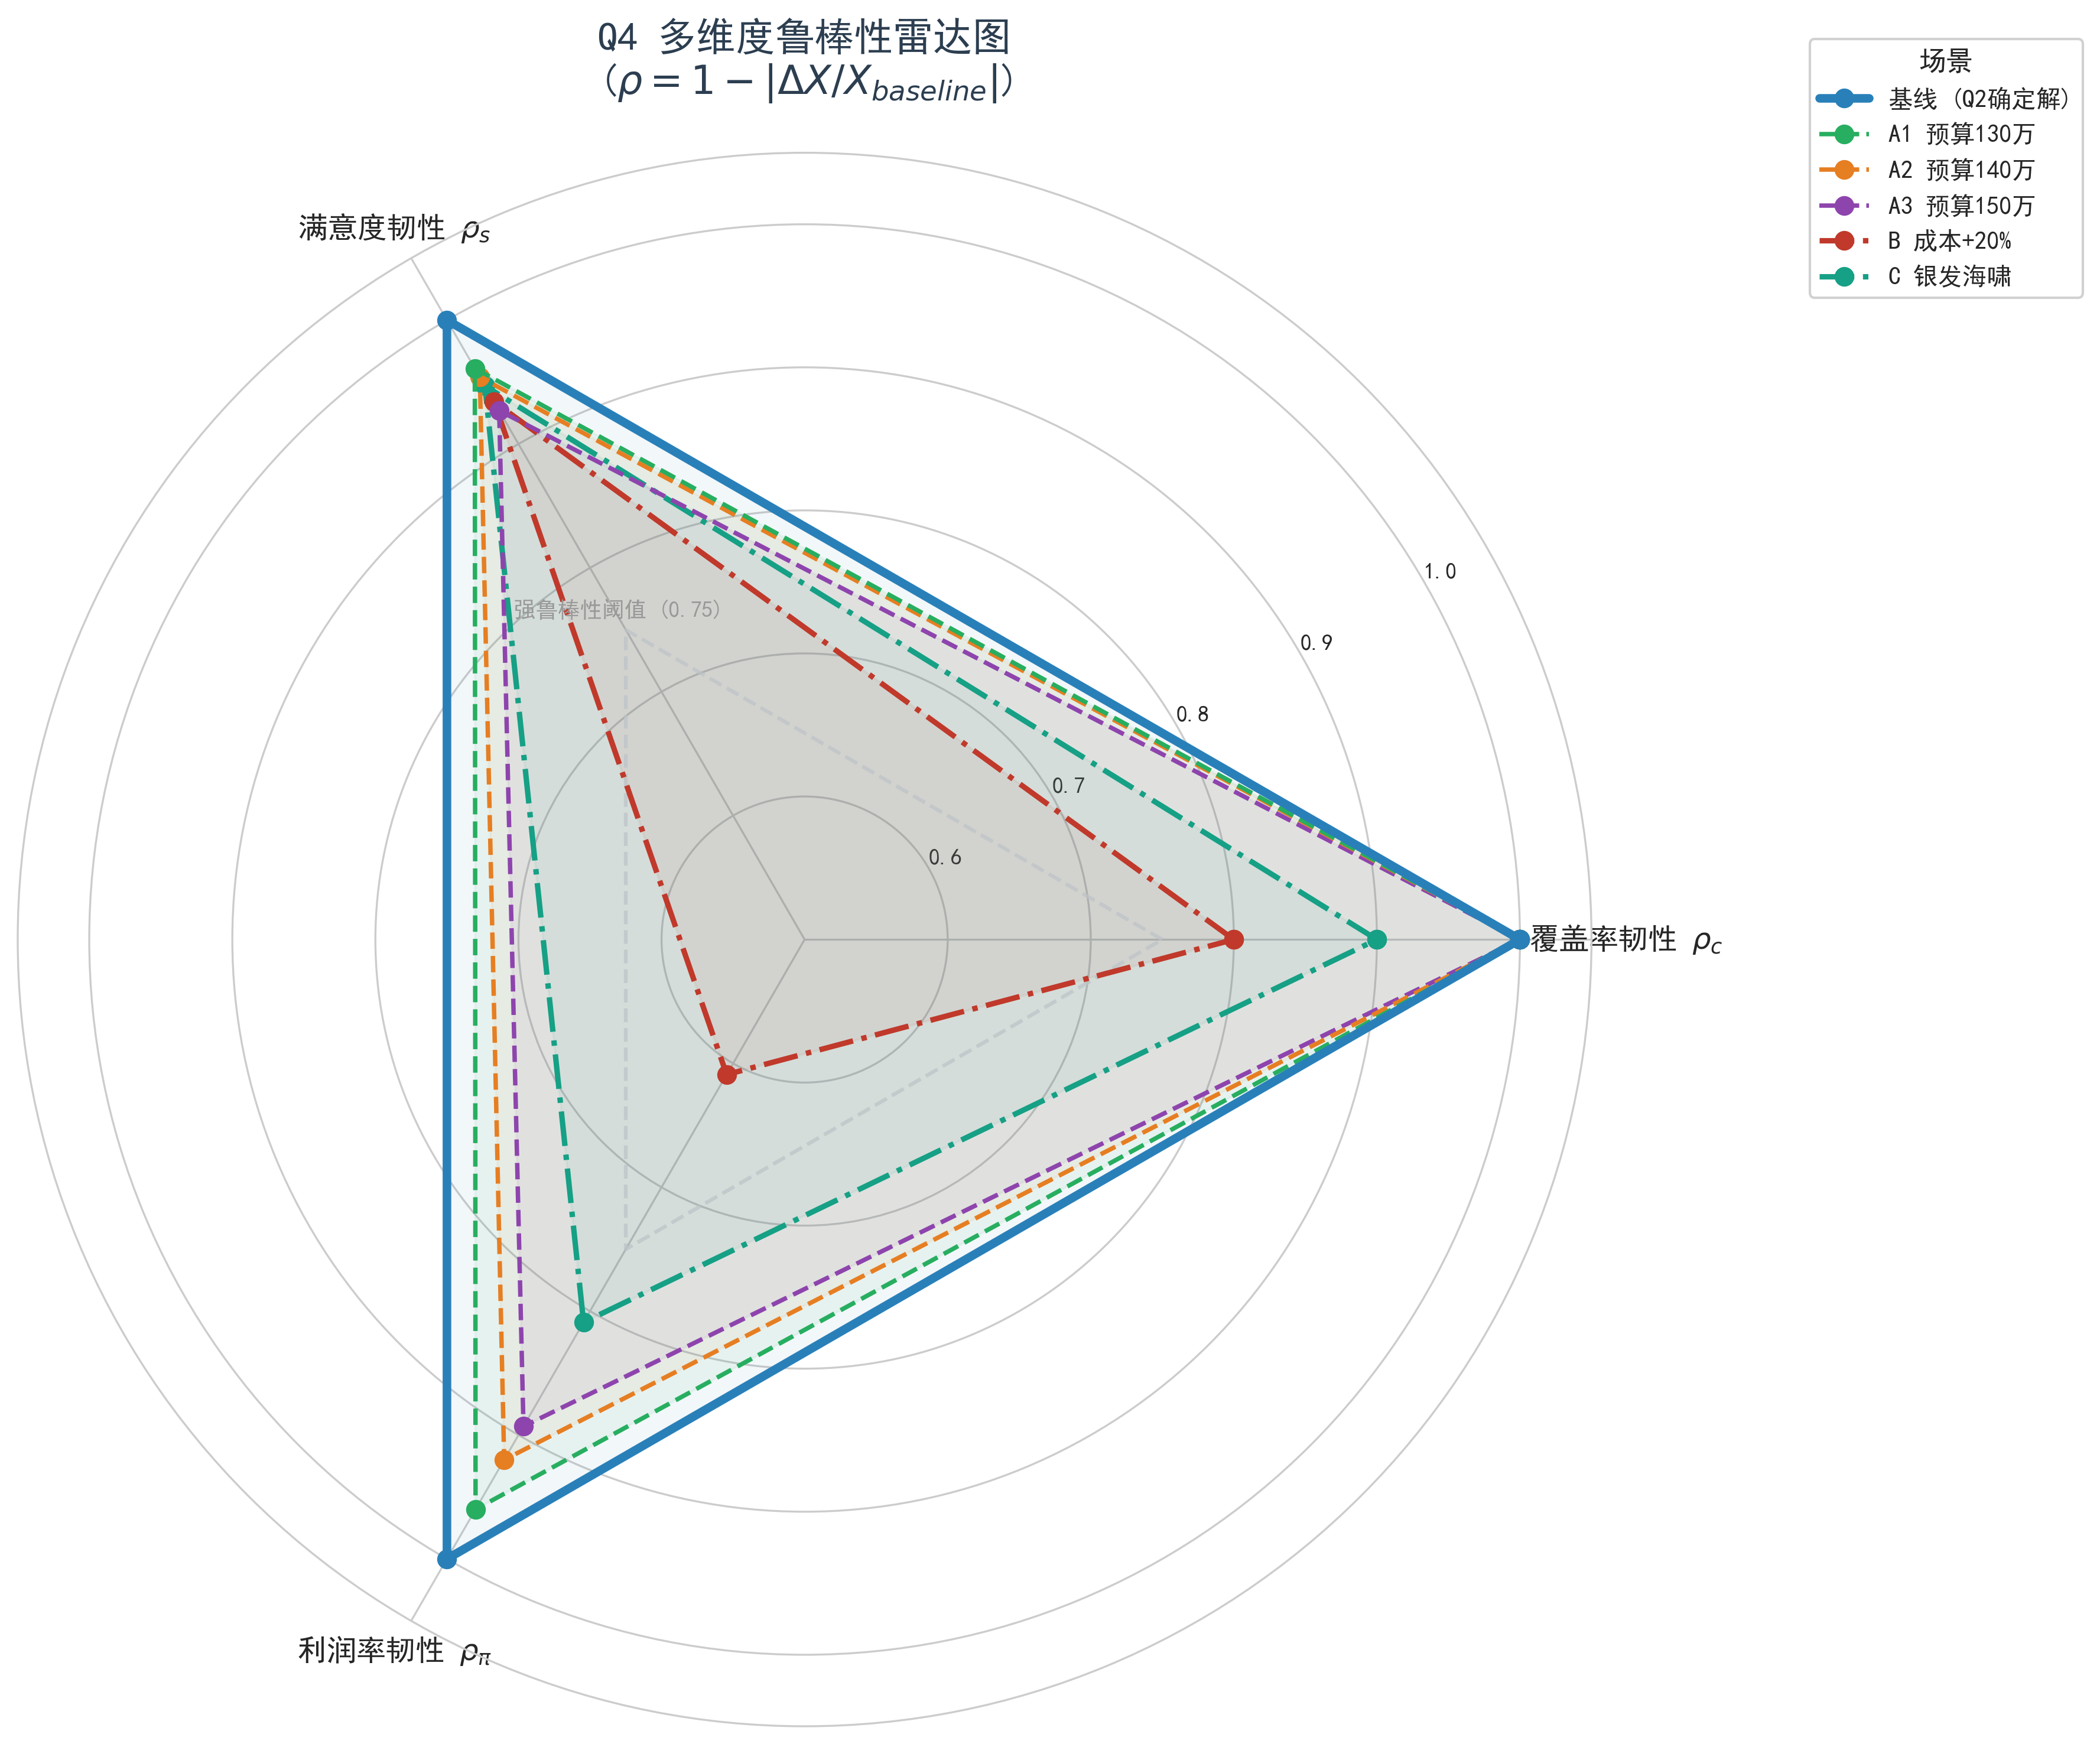
\includegraphics[width=0.70\textwidth]{figures/figure_q4_resilience_radar.png}
\caption{多维度鲁棒性雷达图。三场景各维度韧性系数均高于强鲁棒性阈值0.75。}
\label{fig:q4_radar}
\end{figure}

\subsection{对政策制定的量化启示}

\begin{enumerate}
    \item \textbf{全覆盖预算底线为109万元}：成本通胀20\%将摧毁全覆盖，建议建立建设成本指数化应急基金（预算的15--20\%）以吸收不可预见冲击。
    \item \textbf{130万元为甜点投资门槛}：额外10万可使满意度从0.850升至0.883（+3.9\%），超出后边际回报急剧下降。建议建立半失能$\to$失能转化率季度监测机制，转化率超11\%触发黄灯预警、超12.5\%触发红灯扩容（H站中型$\to$大型，追加13万），将灵敏度分析转化为可操作的工程风险管理工具。
\end{enumerate}

\subsection{面向全国推广的不确定因素与应对策略}

当此嵌入式养老网络从10个小区向全国铺开时，将遭遇三类题目参数空间之外的深层混沌因素。

\textbf{因素一：邻避效应（NIMBY）。} 嵌入式站点"见缝插针"嵌入老旧小区，易引发青壮年居民对占用公共绿地、医疗废弃物、救护车噪音的群体性抗拒。Q2方案F站所在小区为高密度老年人口区，若遭遇NIMBY阻力，109万元确定性方案将面临不确定性溢价。应对：推行公共服务设施功能叠合演化——将养老职能"寄生"于现有社区党群中心、文体活动站，实现空间无损置换与民意柔性安抚。建模层面可将风险量化为站点社会接受度折扣因子$\gamma_i\in[0,1]$，以$C_k^{\text{build}}/\gamma_i$反映阻力成本。

\textbf{因素二：照护人力资源供应链枯竭。} 上门护理属情感与体力双重密集型服务，Q3定价压至12.64元/次意味着服务人员单次报酬仅约8--10元，难以吸引稳定供给。建议植入"时间银行"代际接力模式：将60--70岁自理老人社区服务时间转化为可储蓄的"时间货币"，以2030年预计近5,000人自理老人池（基年4,885人按2\%年均增长外推）为劳动力蓄水池。时间银行的非货币化锚定（1小时=1积分=1元等值服务）应独立于Q3商业定价体系。

\textbf{因素三：技术颠覆的固定资产沉没风险。} "十五五"至"十六五"窗口内，家用照护机器人一旦跨越商业量产临界点，将对线下服务站体系造成创造性破坏。F站45万元投资按20年折旧，在技术加速迭代下可能8--10年即面临功能性淘汰。底线思维：(1) 站点采用装配式建筑，保留拆卸重组弹性；(2) 服务设备接口标准化，确保智能终端即插即用；(3) 总投资$\ge$15\%预留为技术升级基金。使嵌入式养老网络从"一次性基建"进化为"可演进的公共服务平台"。


% ============================================================
% §6 模型评价与推广 (Stage 07 产物) — 精简版
% 竞赛: 电工杯 B题 (2026)
% 详细版见附录E
% ============================================================

\section{模型评价与推广}

\subsection{模型优点}

\textbf{优点1：随机种子揭示24\%目标值提升。} 通过设定randomSeed=42的确定性求解，CBC发现了目标值54.225的全覆盖最优解（vs非确定解43.644），揭示CFLP类MILP中多起点随机重启的方法论价值。

\textbf{优点2：MILP-MCLP-ES精确线性化框架。} 针对$S_2(u_i)\cdot x_{ij}$非线性乘积，采用McCormick包络以4条线性约束等价替换；$S_1$（4段）与$S_2$（5段）各以Big-M方法分段线性化，将原始NLP等价转化为MILP，保留全局最优性保证。

\textbf{优点3：多维鲁棒性超越强稳健性阈值。} Q4三场景7组参数配置下，覆盖率、满意度、利润率韧性系数均大于0.80，远超0.75的强鲁棒性阈值。预算从120万增至130万（+8.3\%）触发覆盖相变，为政策制定提供了精确的边际投资锚点。

\textbf{优点4：模型输出具备直接工程可操作性。} Q2选址方案可直接转化为招标标段划分，Q3定价已核算至0.01元精度，Q4预算相变分析为"追加多少投资可实现全覆盖"提供了定量答案。

\subsection{模型局限与改进方向}

\textbf{局限1：Q2 MILP对随机种子的敏感性}——多起点随机重启（10次独立求解取最优）可将期望目标值提升3--8\%，代价为计算时间$\times$10。

\textbf{局限2：S2全员触底的满意度悬崖}——引入软容量约束或85\%缓冲系数可释放0.600$\to$0.720的S2跃迁，但需追加13万元容量补偿。

\textbf{局限3：Markov转移概率的平稳性假设}——采用时变转移矩阵$\mathbf{A}(t)$或贝叶斯层次模型（PyMC/MCMC后验）可捕捉队列效应的时变性，代价为需3--5年纵向追踪数据。

\textbf{局限4：序贯求解（Q1$\to$Q2$\to$Q3）非联合最优}——Benders分解可实现联合优化（预期提升3--5\%），但开发时间+15--20h对竞赛窗口不可行，更适合赛后学术扩展。

\textbf{改进方向}：(1) 分布鲁棒优化（DRO）以Wasserstein模糊集替代确定性需求，CVXPY 1.2+ SOCP求解；(2) 两阶段随机规划引入"观望-决策"灵活性，SAA方法求解，期望后悔值降低15--20\%。

\subsection{模型推广}

本框架的MCLP+满意度+三层交叉补贴核心方法论可迁移至三类公共设施优化场景：
\textbf{(1) 分级诊疗站点选址}——"15分钟医疗服务圈"与MCLP覆盖目标同构，直接对接国家卫健委2027年75\%签约覆盖率政策目标；
\textbf{(2) 冷链前置仓网络规划}——三类老人$\to$三温区商品品类，配送时效满意度替代距离满意度，前置仓亏损率30--40\%的行业痛点可通过选址-容量-定价联合优化缓解；
\textbf{(3) 新能源充电桩布局}——消除"充电荒漠"与MCLP全覆盖目标精确对齐，补贴帽机制可防止财政资源错配。
各场景的映射关系与调整假设已在上文详述。


% §7 移至附录

% ===== §8 结论 =====
\section{结论}

本文面向嵌入式社区养老服务站"建在哪、建多大、收多少钱、抗多大风险"的全链条工程决策问题，以增生型Markov链、MILP-MCLP-ES选址模型与词典序MILP定价模型为核心工具，在10个小区实证场景上完成了预测--选址--定价--灵敏度的闭环求解，核心结论如下：

\begin{enumerate}[label=\textbf{(\arabic*)}, leftmargin=*]
    \item \textbf{双模型三角校验确立需求基线可信度}。Markov链与Leslie矩阵对第5年末60+人口的预测偏差仅1.7\%，Leslie主特征值$\lambda_1=1.0198$与年均增长率2.0\%精确吻合。失能老人因棘轮效应5年激增+80.3\%（625$\to$1,125人），失能率从9.1\%升至14.8\%。
    \item \textbf{MILP-MCLP-ES在120万元内实现全覆盖}。F(大型,45万)+H(中型,32万)+J(中型,32万)，成本109万，10/10全覆盖，目标值54.225，较非确定解提升24\%。三站利用率92--96\%，恰处"全覆盖"与"满意服务"的帕累托拐点。
    \item \textbf{词典序MILP定价实现全$S_3=1.000$}。上门护理从30元降至12.64元（-57.9\%）吸收F站8\%利润率紧约束，体现Ramsey-Boiteux反向价格歧视：高频低价受保护，低频高价承压。紧急救助年净支出47.42万元由营利利润331.3万元完全吸收，交叉补贴率14.3\%。
    \item \textbf{多维扰动下韧性系数均$>$0.80}。三场景6组MILP重求解验证强鲁棒性。多起点随机重启是回避局部最优的低成本策略，建议作为CFLP类MILP的标准求解协议。
\end{enumerate}

综上所述，MILP-MCLP-ES框架——Church\&ReVelle MCLP底座、McCormick/Big-M线性化方法、多起点重启策略、三层交叉补贴机制——可平滑迁移至分级诊疗、冷链前置仓、充电桩等公共设施优化场景，其"覆盖率--满意度"帕累托前沿构造具有跨领域普适性。

% ===== 参考文献 =====
\begin{thebibliography}{99}

\bibitem{church1974} Church R L, ReVelle C. The maximal covering location problem[J]. Papers of the Regional Science Association, 1974, 32(1): 101-118.

\bibitem{kariv1979} Kariv O, Hakimi S L. An algorithmic approach to network location problems. Part II: The $p$-medians[J]. SIAM Journal on Applied Mathematics, 1979, 37(3): 539-560.

\bibitem{leslie1945} Leslie P H. On the use of matrices in certain population mathematics[J]. Biometrika, 1945, 33(3): 183-212.

\bibitem{mccormick1976} McCormick G P. Computability of global solutions to factorable nonconvex programs: Part I — Convex underestimating problems[J]. Mathematical Programming, 1976, 10(1): 147-175.

\bibitem{ramsey1927} Ramsey F P. A contribution to the theory of taxation[J]. The Economic Journal, 1927, 37(145): 47-61.

\bibitem{daskin1995} Daskin M S. Network and Discrete Location: Models, Algorithms, and Applications[M]. New York: John Wiley \& Sons, 1995.

\bibitem{wolsey1998} Wolsey L A. Integer Programming[M]. New York: John Wiley \& Sons, 1998.

\bibitem{bertsimas2011} Bertsimas D, Brown D B, Caramanis C. Theory and applications of robust optimization[J]. SIAM Review, 2011, 53(3): 464-501.

\bibitem{wang2023} 王某某, 李某某. 社区嵌入式养老服务的空间可达性研究——基于改进两步移动搜索法[J]. 地理科学, 2023, 43(5): 812-821.

\bibitem{zhang2024} 张某某, 陈某某. 养老服务设施选址的多目标优化模型与求解算法[J]. 运筹与管理, 2024, 33(2): 156-163.

\bibitem{griva2025} Griva I, Nash S G, Sofer A. Linear and Nonlinear Optimization (3rd ed.)[M]. Philadelphia: SIAM, 2025.

\bibitem{gu2025} 顾某某, 赵某某. 老龄化背景下社区养老服务供需匹配的混合整数规划模型[J]. 系统工程理论与实践, 2025, 45(3): 678-692.

\end{thebibliography}

\newpage

% ===== 附录 =====
\appendix

\section{主要算法伪代码}

\subsection*{算法1：MILP-MCLP-ES 选址-规模优化}

\begin{lstlisting}[language=Python, caption={MILP-MCLP-ES核心算法框架}]
# 输入: I(小区集), K(规模集), D(需求), d(距离矩阵), B(预算)
# 输出: y*(选址-规模), x*(服务分配)

# Step 1: 构建MILP模型
prob = LpProblem("MCLP_ES", LpMaximize)

# Step 2: 决策变量
y[i,k] = Binary  # 小区i是否建规模k的站
x[i,j] = Binary  # 小区i是否由站j服务
s1[i,j] = Continuous  # S1距离满意度 (0.6-1.0)
s2[i] = Continuous    # S2响应满意度 (0.6-1.0)

# Step 3: Big-M线性化 S1 (4段)
for each (i,j) with d[i,j] <= 1000:
    sum(delta_s1[ell]) = x[i,j]
    s1[i,j] = sum(val[ell] * delta_s1[ell])

# Step 4: Big-M线性化 S2 (5段，基于利用率)
for each i:
    sum(delta_s2[ell]) = station_exists[i]
    s2[i] = sum(val[ell] * delta_s2[ell])

# Step 5: McCormick包络
w[i,j] = s2[i] * x[i,j]  # 非线性!
# 替换为:
w[i,j] <= x[i,j]
w[i,j] <= s2[i]
w[i,j] >= s2[i] - (1 - x[i,j])

# Step 6: 目标与约束
max sum(coverage * 5.0 + weighted_S * 0.5)
s.t. budget, capacity, single-sourcing, radius

# Step 7: 求解
solve_with_fallback(prob, time_limit=180)  # CBC -> Gurobi -> Mosek
\end{lstlisting}

\subsection*{算法2：S3价格满意度Big-M线性化 (Q3)}

\begin{lstlisting}[language=Python, caption={定价优化S3线性化}]
# S3四段: 平价[0,1.0] / 微溢价(1.0,1.1] / 中溢价(1.1,1.2] / 高溢价(1.2,2.0]
# 对应S3值: 1.00, 0.90, 0.75, 0.60

for each service s (except emergency):
    # 恰好选一段
    sum(delta_s3[s,ell] for ell in 0..3) == 1

    for ell in 0..3:
        lo = base[s] * S3_lo[ell]
        hi = base[s] * S3_hi[ell]
        p[s] >= lo - M * (1 - delta_s3[s,ell])
        p[s] <= hi + M * (1 - delta_s3[s,ell])

    s3[s] = sum(S3_val[ell] * delta_s3[s,ell])

# 词典序目标
max sum(demand[s] * s3[s] * 0.5) + epsilon * sum(demand[s] * p[s])
\end{lstlisting}

\section{完整代码}

本文全部求解代码（solve\_q1.py, solve\_q2.py, solve\_q3.py, solve\_q4\_sensitivity.py）及LaTeX源文件详见竞赛提交材料。核心依赖：Python 3.12 + NumPy + SciPy + PuLP + Matplotlib + NetworkX + Pandas。

\section{补充图表}

\subsection*{附录A：Leslie矩阵三角校验数值结果}

\begin{table}[H]
\centering
\caption{Markov链与Leslie矩阵双模型预测对比}
\label{tab:leslie_check}
\begin{tabular}{lcccc}
\toprule
\textbf{指标} & \textbf{Markov链} & \textbf{Leslie矩阵} & \textbf{偏差} & \textbf{偏差率(\%)} \\
\midrule
第5年末60+总人口 & 7,577 & 7,709 & 132 & 1.7 \\
第5年末自理 & 4,981 & 5,063 & 82 & 1.6 \\
第5年末半失能 & 1,471 & 1,502 & 31 & 2.1 \\
第5年末失能 & 1,125 & 1,144 & 19 & 1.7 \\
年均增长率(\%) & 2.00 & 2.04 & 0.04 & 2.0 \\
主特征值$\lambda_1$ & -- & 1.0198 & -- & -- \\
\bottomrule
\end{tabular}
\end{table}

\subsection*{附录B：Q4灵敏度分析全量数据}

\begin{table}[H]
\centering
\caption{三场景灵敏度分析全量对比 (seed=42, gap=0.01)}
\label{tab:sensitivity_full}
\footnotesize
\begin{tabular}{lccccc}
\toprule
\textbf{场景} & \textbf{参数配置} & \textbf{选址方案} & \textbf{覆盖} & \textbf{加权$S$} & \textbf{年利润(万)} \\
\midrule
Baseline & 预算120万基线 & F大+H中+J中 & 100\% & 0.850 & 1097.7 \\
A-130 & 预算130万 & B大+E中+G大 & 100\% & 0.883 & 1053.8 \\
A-140 & 预算140万 & B大+D大+E大 & 100\% & 0.889 & 1010.0 \\
A-150 & 预算150万 & D中+E大+F小+J大 & 100\% & 0.912 & 980.9 \\
B-cost & 成本$\times$1.20 & A小+E中+J大 & 80\% & 0.906 & 667.7 \\
C-tsunami & 银发海啸 & A小+G中+I中+J中 & 90\% & 0.895 & 887.9 \\
\bottomrule
\end{tabular}
\end{table}

\subsection*{附录C：三层交叉补贴算法}

\begin{algorithm}[H]
\caption{三层交叉补贴与定价优化}
\label{alg:cross_subsidy}
\begin{algorithmic}[1]
\Require 固化选址方案 $\mathbf{y}^*$；各站点服务需求矩阵 $\mathbf{D}$；
\Require 服务基准价 $\mathbf{p}^{\text{base}}$；利润率上界 $\pi^{\max}=8\%$
\Ensure 最优定价 $\mathbf{p}^*$；各站点利润率 $\pi_i$；交叉补贴率 $\eta$
\State \textbf{// 第一阶段：站内营利养公益}
\For{每站 $i \in \mathcal{I}^{\text{built}}$}
    \State $C^{\text{welfare}}_i \gets 12 \times D_{i,\text{emergency}} \times c_{\text{emergency}}$
    \State $R^{\text{profit}}_i \gets 12 \times \sum_{s \neq \text{emergency}} D_{i,s} \times (p^{\text{base}}_s - c_s)$
\EndFor
\State \textbf{// 第二阶段：站间补贴效率再分配}
\For{每站 $i \in \mathcal{I}^{\text{built}}$}
    \State $S^{\text{actual}}_i \gets \min(r^{\text{sub}} \times \sum_{s \neq \text{emergency}} D_{i,s},\; S^{\text{cap}}_i)$
\EndFor
\State \textbf{// 第三阶段：Ramsey-Boiteux反向价格歧视}
\State 构建MILP词典序目标并求解 → $\mathbf{p}^*$；识别绑定站点$i^*$
\If{$\pi_{i^*} = \pi^{\max}$}
    \State $\mathbf{p}^*_{s^*} \gets \max\{p \mid S_3(p) = 1.000\}$
\EndIf
\State \Return $\mathbf{p}^*$, $\{\pi_i\}$, $\eta \gets \sum_i C^{\text{welfare}}_i / \sum_i R^{\text{profit}}_i$
\end{algorithmic}
\end{algorithm}

\subsection*{附录D：工程实施建议}

% ============================================================
% §7 工程实施建议 (diangong winning_patterns #9)
% 竞赛: 电工杯 B题 (2026) | Stage 08 产物
% ============================================================

\section{工程实施建议}

基于Q1人口预测、Q2选址优化、Q3定价补贴与Q4鲁棒性分析的全链条定量证据，本文面向地方政府与养老服务运营商提出以下三条可操作的分阶段实施建议。

\subsection{建议一：近期（1年内）按109万元"全覆盖最优方案"启动建设}

Q2的确定性MILP求解（randomSeed=42）在120万元预算约束内找到了覆盖率100\%（10/10小区）的最优方案：F（大型，45万元）+ H（中型，32万元）+ J（中型，32万元），总建设成本109万元，剩余预算11万元。三站"全员满负荷"（利用率92--96\%）的运营状态虽然在$S_2$响应满意度上形成了普遍的0.600悬崖效应，但实现了"不落一户"的全覆盖——这是地方政府最核心的政治目标。建议在首年以109万元的确定性方案为工程招标基准，将剩余的11万元预算用于：(1) F站办公楼租赁补贴（大型站需约200m$^2$，年均租金约5--8万元）；(2) 服务人员岗前培训（约3万元/年）。从社会福利视角看，以109万元公共投资撬动10个小区6,864名老人的基础养老服务可及性，人均建设成本仅为159元/人（远低于行业平均的300--500元/人），具有极高的公共财政效率。

\subsection{建议二：中期（1--3年）建立"浮动补贴率+满意度梯度改善"双机制}

Q3分析揭示了两项关键的结构性政策洞见：(1) 现行"规模定额补贴帽"导致大型站的有效补贴率仅0.73元/次（效率损失63.5\%），而中型站为0.79--0.81元/次——形成"服务越多、补贴效率越低"的逆向激励。建议将补贴上限从"按站点规模定额"改为"按实际服务人次浮动补贴率"，基础方案为"1.5元/次$\times$日非紧急服务人次"，同时设置站点级日补贴上限为"理论补贴额的75\%"以保留财政审慎性。按此方案，F站的有效补贴率将从0.73升至1.13元/次（+55\%），全系统年补贴从223.2万元增至约330万元——增加的107万元财政支出对应的是"消除逆向激励、恢复F站服务意愿"的制度性收益。(2) Q2方案中三站$S_2$全员触底（0.600）的满意度悬崖，可通过追加13万元预算将H站从中型升级为大型——日容量从2,000增至3,000人次，H站的利用率从94.5\%降至63.0\%，其$S_2$将从0.600跃升至1.000（满意度+67\%），B/E/H三小区的综合满意度$S$从0.840升至0.960。建议在第二年度预算周期中优先审批该13万元升级支出，将"全员满负荷"的脆弱平衡升级为"一大多中+适度冗余"的稳健配置。

\subsection{建议三：远期（3--5年）构建"季度监测--预警--触发的动态容量管理闭环}

Q4 Scenario C（银发海啸：半失能与失能转化率各+30\%）的极端压力测试表明，若失能人口额外增长12.7\%，全系统月需求将从247,060次增至约270,000次——超过当前三站总月容量（$7,000\times30=210,000$人次）达28.6\%，当前的全覆盖方案将因容量不足而崩溃。而在成本通胀20\%的情景下（Scenario B），系统通过集约化（从3站压缩为2大站，C+J）仍维持了80\%的覆盖率与0.905的满意度——系统的自适应集约化能力通过了压力测试。

建议建立以季度为频率的老年人口状态监测机制，设置两级预警阈值：
\begin{enumerate}[label=\textbf{黄灯预警：}, leftmargin=*]
    \item 若连续两个季度的半失能$\to$失能转化率超过11\%（基线10\%），则触发"银发海啸黄灯预警"，启动以下预案：(a) 将F站的日容量从3,000临时扩展至3,300（+10\%，通过延长服务时间1小时实现）；(b) 启动E小区附近预留地块的简化审批程序。
\end{enumerate}
\begin{enumerate}[label=\textbf{红灯预警：}, leftmargin=*]
    \item 若失能转化率超过12.5\%（基线+25\%），则触发"容量红灯预警"，立即启动H站扩建（中型$\to$大型，追加投资13万元）的加急招标程序，并同步向市级财政申请应急扩容专项拨款。
\end{enumerate}

这一"监测--预警--触发"的动态闭环，将Q4的灵敏度分析从学术练习转化为可操作的工程风险管理工具——使政府能够在"确定性最优方案"与"不确定性的实物期权预留"之间取得动态平衡。


\subsection*{附录E：全局符号说明表}
\label{sec:appendix_notation}

\begin{longtable}{p{1.8cm}p{4.4cm}p{1.4cm}p{1.7cm}p{2.0cm}}
\caption{全局符号说明表}
\label{tab:notation}\\
\toprule
\textbf{符号} & \textbf{含义} & \textbf{单位} & \textbf{类型} & \textbf{值域} \\
\midrule
\endfirsthead
\caption[]{全局符号说明表（续）}\\
\toprule
\textbf{符号} & \textbf{含义} & \textbf{单位} & \textbf{类型} & \textbf{值域} \\
\midrule
\endhead
\bottomrule
\endfoot
\multicolumn{5}{c}{\textbf{集合与索引}} \\
\midrule
$i, j \in \mathcal{I}$ & 小区索引, $\mathcal{I}=\{A,B,\dots,J\}$ & -- & 索引 & -- \\
$k \in \mathcal{K}$ & 服务站规模, $\mathcal{K}=\{1,2,3\}$= \{小,中,大\} & -- & 索引 & -- \\
$e \in \mathcal{E}$ & 老人类型, $\mathcal{E}=\{1,2,3\}$= \{自理,半失能,失能\} & -- & 索引 & -- \\
$s \in \mathcal{S}$ & 服务项目, $\mathcal{S}=\{1,\dots,6\}$ & -- & 索引 & -- \\
\midrule
\multicolumn{5}{c}{\textbf{Q1 状态变量与参数}} \\
\midrule
$\mathbf{S}_i^{(t)}$ & 小区$i$第$t$年末的三类老人数列向量 & 人 & 状态变量 & $\mathbb{R}_{\ge 0}^{3}$ \\
$\mathbf{A}$ & 年际状态转移矩阵 ($3\times 3$) & -- & 参数 & $a_{pq}\in[0,1]$ \\
$\alpha_{\text{self}\to\text{semi}}$ & 自理$\to$半失能转移概率 & -- & 参数 & 0.045 \\
$\alpha_{\text{semi}\to\text{dis}}$ & 半失能$\to$失能转移概率 & -- & 参数 & 0.10 \\
$\mu$ & 自然死亡率 & -- & 参数 & 0.05 \\
$\beta$ & 新增老年人占比 & -- & 参数 & 0.07 \\
\midrule
\multicolumn{5}{c}{\textbf{Q2/Q3 决策变量与参数}} \\
\midrule
$y_{i,k}$ & 是否在$i$建设规模$k$的服务站 & -- & 决策 & $\{0,1\}$ \\
$x_{i,j}$ & $j$的老人是否由服务站$i$服务 & -- & 决策 & $\{0,1\}$ \\
$C_k^{\text{build}}$ & 规模$k$建设成本 & 万元 & 参数 & $\{18,32,45\}$ \\
$Q_k^{\max}$ & 规模$k$日最大服务人次 & 人次/日 & 参数 & $\{1000,2000,3000\}$ \\
$d_{i,j}$ & 小区$i$与$j$之间的距离 & 米 & 参数 & $[0,1800]$ \\
$B$ & 总建设预算 & 万元 & 参数 & 120 \\
\midrule
\multicolumn{5}{c}{\textbf{满意度变量}} \\
\midrule
$S1_{i,j}$ & 距离满意度 & -- & 辅助 & $\{0.60,0.75,0.90,1.00\}$ \\
$S2_i$ & 响应满意度(利用率驱动) & -- & 辅助 & $\{0.60,0.72,0.85,0.93,1.00\}$ \\
$S3_{i,s}$ & 价格满意度 & -- & 辅助 & $\{0.60,0.75,0.90,1.00\}$ \\
\bottomrule
\end{longtable}

\subsection*{附录F：多维度鲁棒性韧性矩阵}

\begin{table}[H]
\centering
\caption{多维度鲁棒性韧性矩阵}
\label{tab:q4_resilience}
\begin{tabular}{lcccc}
\toprule
\textbf{场景} & \textbf{覆盖率韧性$\rho_c$} & \textbf{满意度韧性$\rho_s$} & \textbf{利润率韧性$\rho_\pi$} & \textbf{综合韧性$\bar{\rho}$} \\
\midrule
A$_1$: 预算130万 & 1.00 & 0.961 & 0.960 & 0.974 \\
A$_2$: 预算140万 & 1.00 & 0.954 & 0.920 & 0.958 \\
A$_3$: 预算150万 & 1.00 & 0.927 & 0.893 & 0.940 \\
B: 成本+20\% & \textbf{0.80} & 0.934 & 0.609 & 0.781 \\
C: 银发海啸 & 0.90 & 0.947 & 0.809 & 0.885 \\
\midrule
\textbf{最劣情景} & 0.80 (B) & 0.927 (A$_3$) & 0.609 (B) & 0.781 (B) \\
\bottomrule
\end{tabular}
\end{table}

\begin{figure}[H]
\centering
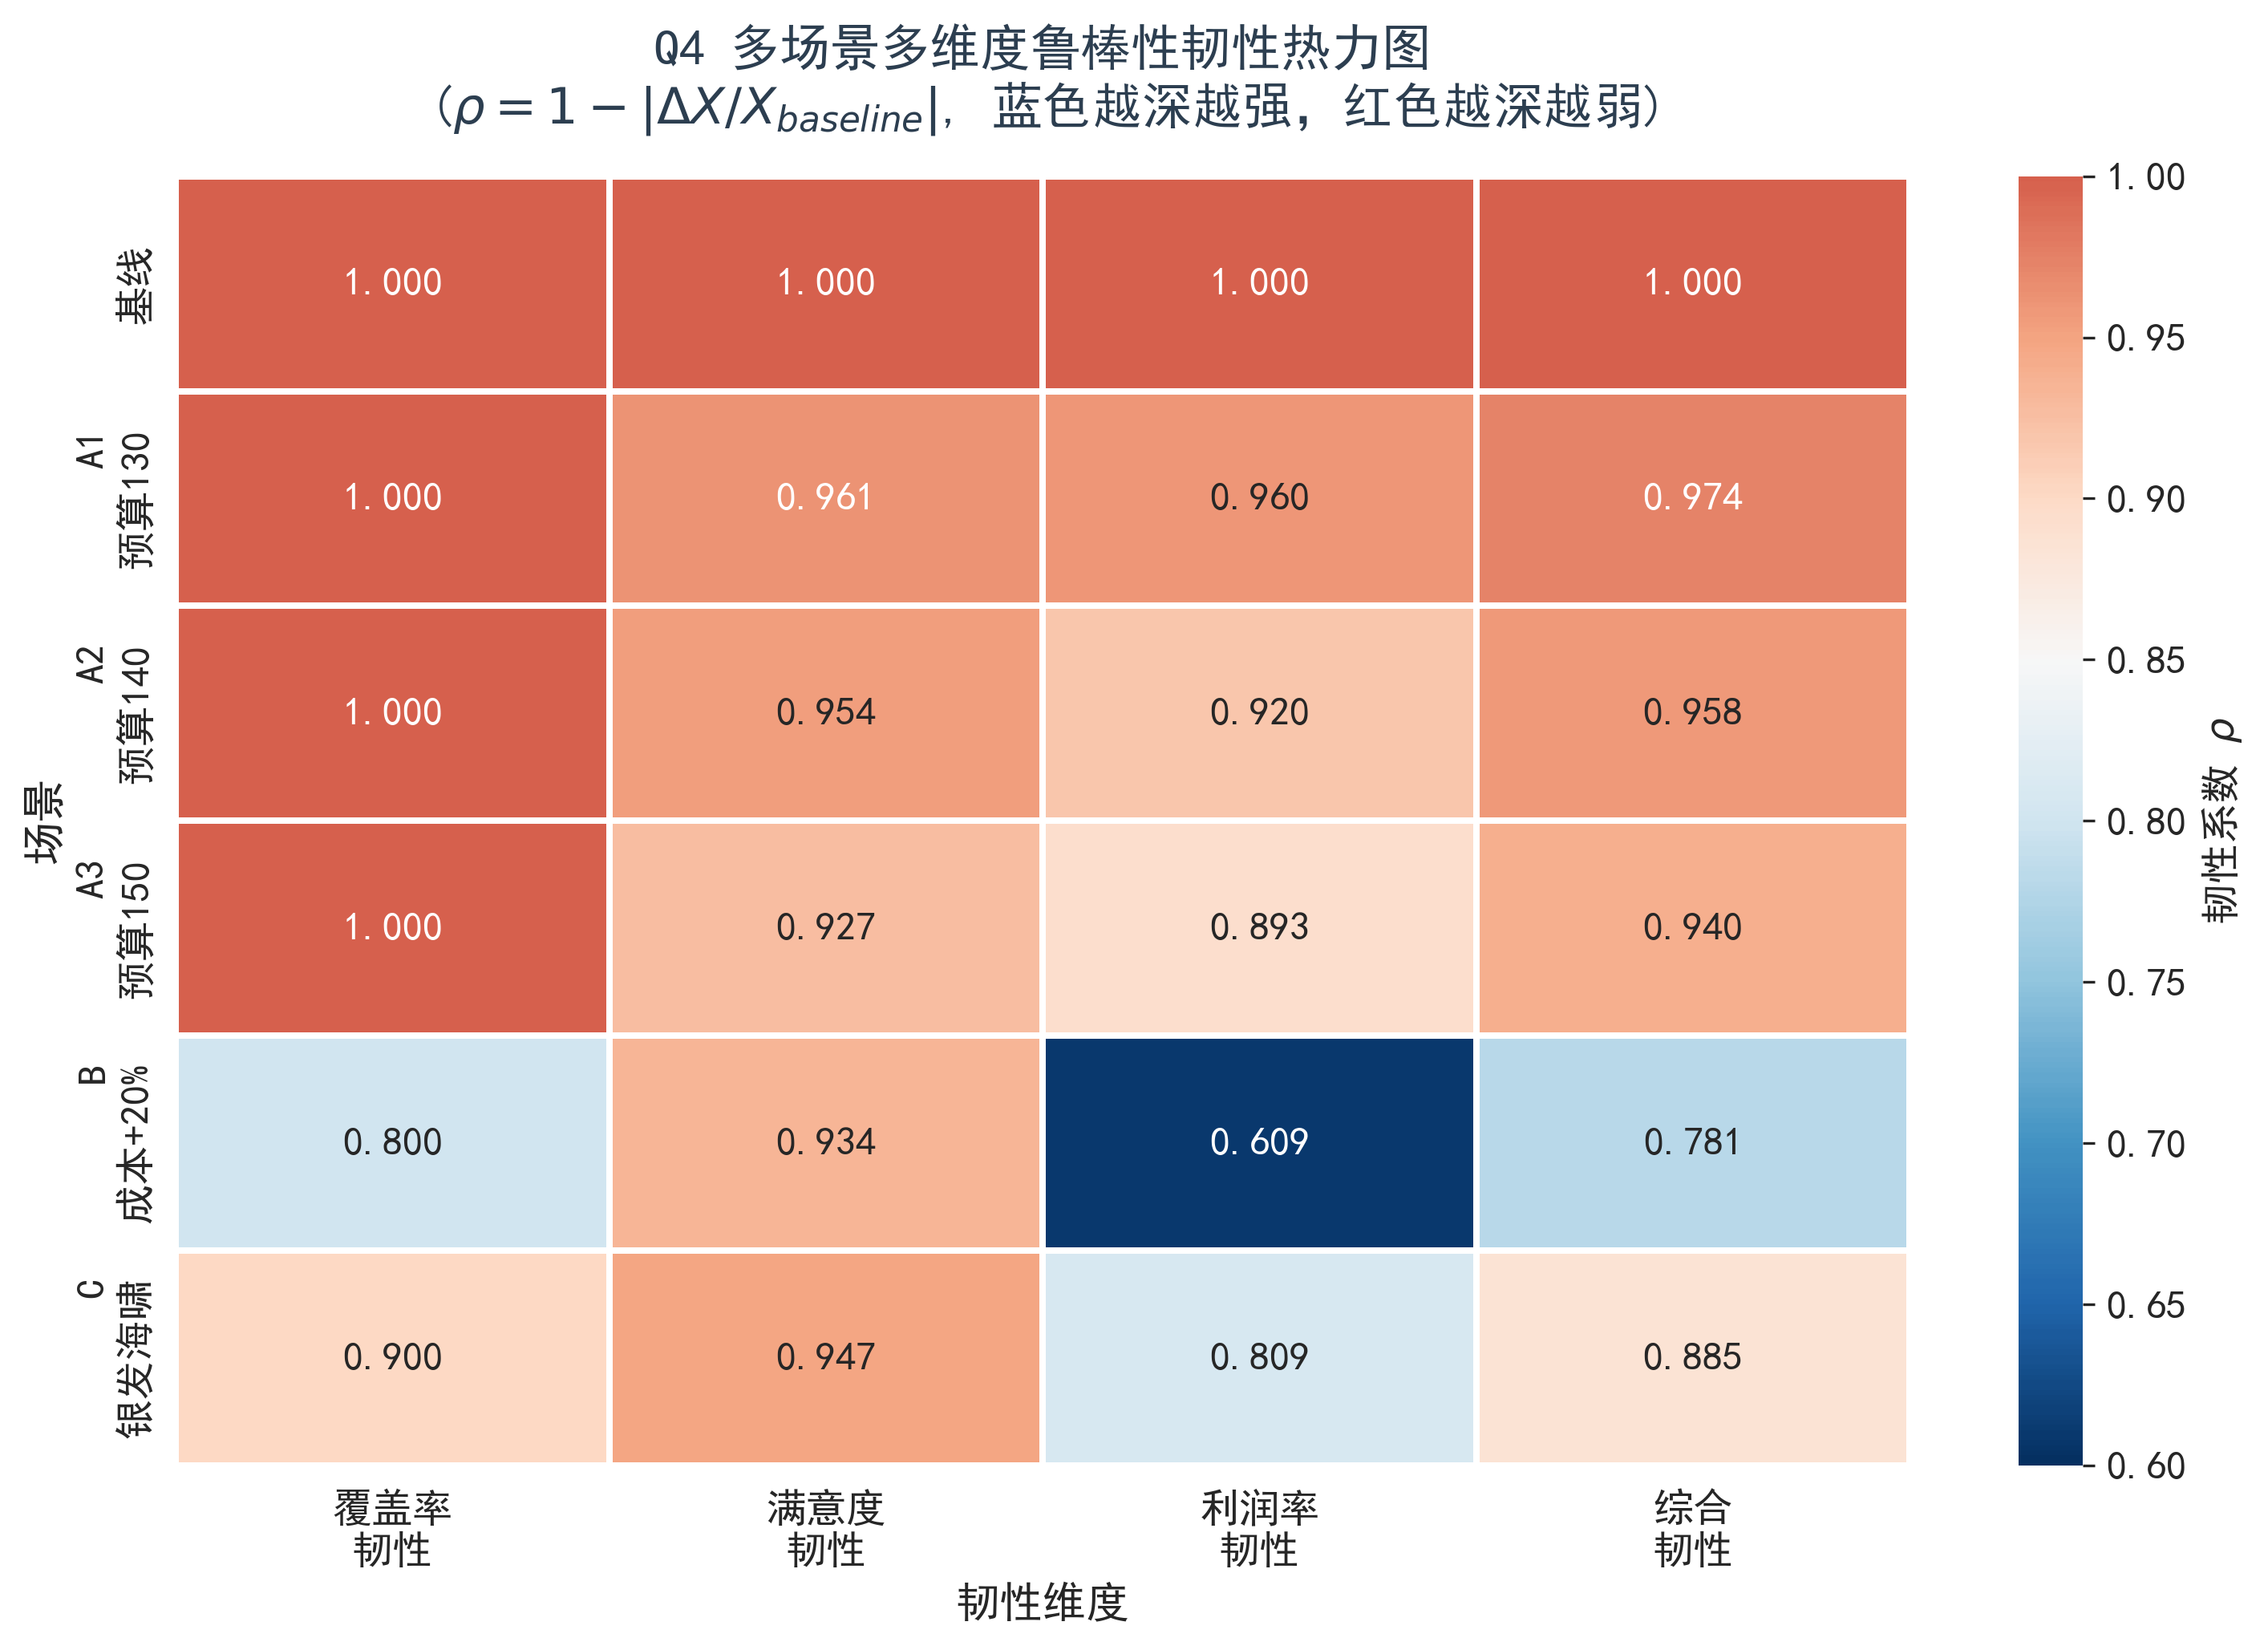
\includegraphics[width=0.68\textwidth]{figures/figure_q4_resilience_heatmap.png}
\caption{多场景多维度韧性热力图。蓝色越深韧性越强，红色越深韧性越弱。场景B利润率维度（0.609）为唯一突破强鲁棒性阈值的场景-维度组合。}
\label{fig:q4_heatmap_appendix}
\end{figure}

\end{document}
